% (English follows)
% Questo gruppo di 7 file .tex \`e stato creato nel Giugno 2015 da Elisa Davoli e Matteo Tommasini per il loro matrimonio.
% Usatelo liberamente per il vostro matrimonio! Nel caso voleste ridistribuire le vostre modifiche, vi preghiamo di citare la pagina
% blognotes.matteotommasini.altervista.org/latex-matrimonio come referenza.
% Questo lavoro \`e distribuito con licenza CC-BY (potete copiare, distribuire e creare lavori derivati a partire da questo, a patto
% di citare questo blog per il lavoro originale).
% L'intero codice \`e rilasciato ``as it is'', senza nessuna garanzia di buon funzionamento (nel nostro caso funzionava alla perfezione!).
% I pdf compilati (pagina singola e pagina doppia) si possono scaricare alla stessa pagina menzionata sopra.
% L'unico pacchetto usato qui e che non trovate in una distribuzione standard di LaTeX \`e il pacchetto pgfornament (istruzioni nel file n. 1).
% Una buona guida per l'installazione di pgfornament in debian e derivate \`e questa:
% https://toihoctap.wordpress.com/2013/02/24/install-package-pgfornament-for-texlive-2012-in-ubuntu-12-04-lts/
% Il manuale del pacchetto pgfornament è disponibile qui:
% http://altermundus.com/pages/downloads/packages/pgfornament/ornaments.pdf
% L'unica imprecisione del manuale di pgfornament \`e che il pacchetto è sempre chiamato ``ornament'' invece che ``pgfornament''.
% Il pdf creato con questa serie di 7 file \`e la versione che abbiamo usato per il nostro matrimonio. A seconda delle letture e delle formule
% scelte per il rito, il libretto della vostra messa potr\`a differire in maniera significativa da questo. Questo \`e solo una (si spera utile)
% guida per voi! Per la scelta completa di tutte le letture e le formule del rito, vi rimandiamo direttamente al libretto della messa degli sposi,
% disponibile in ogni parrocchia cattolica. Alcune parti del rito sono nuove in italiano e non esiste ad oggi (Giugno 2015) una traduzione ufficiale. Quindi
% nella versione inglese alcune parti sono tradotte da noi. Se vi serve la versione inglese, controllate se \`e uscita una traduzione ufficiale!
%%%
% This group of 7 .tex files was created in June 2015 by Elisa Davoli and Matteo Tommasini for their wedding.
% Use it freely for your wedding. If you want to redistribuite your changes to this code, please cite
% blognotes.matteotommasini.altervista.org/latex-matrimonio as a reference
% The license is the standard CC-BY (you can copy, distribute and make derivative works based on this work,
% provided that you give credit to this blog for the original work).
% The entire code is provided ``as it is'', without any warranty (in our case it worked perfectly!).
% The compiled pdfs (single and double page) can be downloaded from the same webpage mentioned above.
% The only package that is used here and that is not part of a standard LaTeX distribution is the package pgfornament (instructions in the file n. 1).
% A good guide for the installation of pgfornament in debian/ubuntu/etc is the following one:
% https://toihoctap.wordpress.com/2013/02/24/install-package-pgfornament-for-texlive-2012-in-ubuntu-12-04-lts/
% You can download the manual of the package pgfornament from here:
% http://altermundus.com/pages/downloads/packages/pgfornament/ornaments.pdf
% The only error of the pgfornament manual is the fact that the package is always refered to as ``ornament'' instead of ``pgfornament''.
% The pdf created from this series of 7 files is the version that we used for our wedding. Depending on the lectures, the gospel and the different
% parts of the rite that you can choose, your booklet can vary significantly from this one. This booklet is only a (hopefully useful) guide for you!
% For the complete choices of lectures and parts of the rite, please refer directly to the booklet of the mass with wedding that you can find in any
% catholic parish. In June 2015 some parts of the rite were new in Italian, and not yet officially translated in English, so we translated them. If you
% need the English version of the booklet, please check if the official translation is already out.

\documentclass[11pt]{book}
\usepackage{etoolbox} % package needed for the toggle commands below

\newtoggle{bookletprinting} % pagina doppia (versione finale) o pagina singola (debug version)
\newtoggle{debugmode} % debug mode on or off
\newtoggle{pgfornamentinstalled} % pacchetto pgfornament installato sul vostro computer oppure no
\newtoggle{italianlanguage} % lingua italiana
\newtoggle{englishlanguage} % lingua inglese

% CAMBIATE I VALORI (true/false) DEI SEGUENTI TOGGLE A VOSTRO PIACIMENTO.
%%%
% PLEASE CHANGE THE VALUES (true/false) OF THE NEXT TOOGLES IF YOU NEED TO.

\toggletrue{bookletprinting} % opzioni: \toggletrue per l'impaginazione a libretto (booklet), \togglefalse per l'impaginazione a pagina singola
% l'opzione true deve essere usata solo quando avete gi\`a sistemato tutti i canti, le letture e le formule del rito. Prima vi conviene usare
% l'opzione false. Il risultato non \`e perfetto nella pagina, ma \`e pi\`u comodo da usare quando un testo \`e diviso su pi\`u pagine.
%%%
% Options: \toggletrue for printing a booklet, \togglefalse in order to have a pdf with one page per sheet (``single page'' mode). You should use the
% option \toggletrue only after having written all the songs, the lectures, etc. Before that it is much simpler to use the option \togglefalse

% La seconda pagina della versione ``booklet'' \`e intenzionalmente bianca, in modo tale da avere il testo che
% cominci sulla pagina destra e l'ultima pagina bianca. Questo equivale a 2 pagine bianche nella versione ``a pagina singola'' (la seconda e la penultima).
% Se le pagine totali della versione ``a pagina singola'' non sono divisibili per 4, allora avrete alcune pagine bianche extra. Per capire quali sono le
% pagine bianche extra, \`e conveniente usare la modalit\`a di debug qui sotto.
%%%
% The second page of the ``booklet'' version is blank on purpose: in this way the text starts on a page on the right and the last page is blank. This
% is equivalent to having 2 white pages in the version ``single page'' (the second one and the second last one). If the total number of pages
% in the ``single page'' mode is not divisible by 4, you will have some more blank pages. If you need to understand which are the extra blank pages,
% you should use the debug mode below

\togglefalse{debugmode} % opzioni: true: aggiunge la scritta ``PAGINA LASCIATA VOLONTARIAMENTE BIANCA - NEL MAIN FILE CAMBIARE ``DEBUGMODE''
% IN ``FALSE'' PRIMA DI STAMPARE DEFINITIVAMENTE IL LIBRETTO!'' sulla seconda e sulla penultima pagina
% false: crea solo la pagina bianca, senza scritte aggiuntive (usare questa versione per la stampa finale)
%%%
% options: true: it adds the text ``THIS PAGE IS INTENTIONALLY LEFT BLANK - IN THE MAIN FILE CHANGE ``DEBUGMODE''
% TO ``FALSE'' BEFORE PRINTING THE FINAL VERSION OF THE BOOKLET!`` on the second and on the second last page
% false: creates only a blank page, without additional text (use this version for the final printing)

\togglefalse{pgfornamentinstalled} % opzioni: \toggletrue, se siete riusciti ad installare il pacchetto pgfornament,
% \tooglefalse in caso contrario (tutti gli ornamenti che vedete nel pdf di esempio non saranno stampati).
%%%
% Options: \toogletrue if you managed to install the package pgfornament on your computer -
% \tooglefalse on the opposite case (all the ornaments that you see in the sample pdf will not be printed).

\togglefalse{italianlanguage} % opzioni: \toggletrue per la lingua italiana, \tooglefalse per non avere la lingua italiana
%%%
% Options: \toggletrue for the italian language, \tooglefalse for not having the italian language

\toggletrue{englishlanguage} % opzioni: \toggletrue per la lingua inglese, \tooglefalse per non avere la lingua inglese.
%%%
% Options: \toggletrue for the english language, \tooglefalse for not having the english language

% ATTENZIONE: ogni volta che compilate dovete scegliere solo una lingua tra italiano ed inglese!
%%%
% ATTENTION: every time that you compile, you have to choose only one language between Italian ans English!

\ifboolexpr{togl{italianlanguage} and togl{englishlanguage}}
% Se il test passa, allora entrambe le lingue sono state selezionate
%%%
% If the test is true, then both languages were selected
{\begin{document} ATTENZIONE! HAI SELEZIONATO CONTEMPORANEAMENTE SIA L'ITALIANO SIA L'INGLESE. Nel main file devi scegliere due valori di verit\`a
diversi per la lingua italiana e per la lingua inglese. Ritenta e sarai pi\`u fortunato :-) \\

ATTENTION! YOU HAVE SELECTED BOTH ITALIAN AND ENGLISH AS A MAIN LANGUAGE. In the main file you have to select 2 different truth values for
Italian and English. Try again and you'll have more luck :-)\end{document}}
{\ifboolexpe{not (togl{italianlanguage} or togl{englishlanguage})}
% Se questo test secondario passa, allora nessuna lingua era selezionata
%%%
% If this auxiliary test is true, then no language was selected
 {\begin{document} ATTENZIONE! NON HAI SELEZIONATO NESSUNA LINGUA (ITALIANO O INGLESE). Nel main file devi scegliere true per la lingua italiana e false
 per la lingua inglese, o viceversa. Ritenta e sarai pi\`u fortunato :-) \\

 ATTENTION! YOU HAVE NOT SELECTED ANY LANGUAGE (ITALIAN OR ENGLISH). In the main file you have to select true for Italian and false for English,
 or conversely. Try again and you'll have more luck :-)\end{document}}
% Se tutti i test precedenti hanno fallito, allora abbiamo scelto un'unica lingua (italiano o inglese). Si comincia il codice principale
%%%
% If all the previous tests are negative, then we have chosen exactly one language (Italian or English). So we can start the main code
 {
 % Nome degli sposi
%%%
% Name of the bride and groom
\newcommand{\bride}{Elisa}
\newcommand{\groom}{Matteo}

% nome della santa della sposa e invocazione
%%%
% name of the patron saint of the bride and invocation
\iftoggle{italianlanguage}
  {\newcommand{\patronsaintofthebride}{\textrm{Sant'Elisa} & \textbf{prega per noi}}}{}
\iftoggle{englishlanguage}
  {\newcommand{\patronsaintofthebride}{\textrm{Saint Elisa} & \textbf{pray for us}}}{}

% nome del santo dello sposo e invocazione
%%%
% name of the patron saint of the groom and invocation
\iftoggle{italianlanguage}
  {\newcommand{\patronsaintofthegroom}{\textrm{San Matteo} & \textbf{prega per noi}}}{}
\iftoggle{englishlanguage}
  {\newcommand{\patronsaintofthegroom}{\textrm{Saint Mathew} & \textbf{pray for us}}}{}

% nome del santo/santa della chiesa e invocazione
%%%
% name of the patron saint of the church and invocation
\iftoggle{italianlanguage}
  {\newcommand{\patronsaintofthechurch}{\textrm{San Silvestro} & \textbf{prega per noi}}}{}
\iftoggle{englishlanguage}
  {\newcommand{\patronsaintofthechurch}{\textrm{Saint Sylvester} & \textbf{pray for us}}}{}

% risposta alla preghiera dei fedeli
%%%
% answers for the prayers of the faithful
\iftoggle{italianlanguage}
  {\newcommand{\answerforprayers}{Ascoltaci, o Signore.}}{}
\iftoggle{englishlanguage}
  {\newcommand{\answerforprayers}{Lord, hear our prayer.}}{}

% nome del vescovo della diocesi
%%%
% name of the bishop of the diocese
\iftoggle{italianlanguage}
  {\newcommand{\nameofbishop}{Carlo}}{}
\iftoggle{englishlanguage}
  {\newcommand{\nameofbishop}{Carlo}}{}
  
% nome del papa
%%%
% name of the pope
\iftoggle{italianlanguage}
  {\newcommand{\nameofpope}{Francesco}}{}
\iftoggle{englishlanguage}
  {\newcommand{\nameofpope}{Francis}}{}

% colore per il titolo dei canti (compresi gli ornamenti a destra e a sinistra)
%%%
% color for the titles of the songs and for the ornaments on the left and right of such titles
\def \songstitlecolor {black!60}

% colore per i testi dei canti
%%%
% color for the text of the songs
\def \textofsongcolor {black!80}

% colore per il nome del celebrante, dell'assemblea, degli sposi, per il segno della croce,
% per i capitelli nelle 2 letture e nel Vangelo, per gli header e per gli header su 2 linee
%%%
% Color fo the name of the celebrant, the assembly, the bride and the groom, the maltese cross,
% the big initials for the 2 readings and the Gospel, for the headers and for the headers on 2 lines
\def \maincolor {red} % comprende i nomi degli sposi, del vescovo della diocesi, del papa,
 % le risposte alla preghiera dei fedeli, alcuni colori modificabili facilmente, etc
 %%%
 % contains the name of the bride and groom, of the bishop, of the pope, the answers to the prayer of the faithful, some tweaks about colors, etc 
 
 \usepackage[utf8]{inputenc} % 5 pacchetti standard % 5 standard packages
\usepackage[T1]{fontenc}
\usepackage[italian]{babel}
\usepackage{indentfirst}
\usepackage{graphicx} % per tagliare i margini dell'immagine sull'ultima di copertina % this is used for adjusting the margins on the back cover
\usepackage[export]{adjustbox} % per aggiungere il bordo all'immagine sull'ultima di copertina % this is used for adding a border to the image on the back cover
\usepackage{xcoffins} % per fare i titoli delle sezioni % this is used for creating the titles of the various section
\usepackage{emerald} % per avere il font usato nella copertina per i nomi degli sposi % this is used for the font used for the bride and groom on the front page
\usepackage{accanthis} % per avere \accanthis, font usato nella copertina per tutte le altre scritte % this is used for the font \accanthis, used for everything else in the front page
\usepackage{harmony} % serve per avere \textsc, usato per il font secondario nei titoli delle letture % this is used for \textsc, used for the secondary font in the titles of the lectures
\usepackage{pict2e} % per avere \textscm, usato per il font del celebrante, dell'assemblea e degli sposi % this is used for the font \textscm (for the celebrant, the bride and groom and the assembly)
\usepackage{lettrine} % per fare le iniziali grandi nelle 2 letture e nel vangelo % for the big initials in the 2 lectures and in the gospel
\usepackage{tikz} % per fare la copertina con tikzpicture % used for creating the front page with tikzpicture
\usepackage{ifthen} % per passare facilmente dalla versione italiana a quella inglese e per passare da pagina singola a pagina doppia
% used in order to switch from the Italian to the English version, and from the single page to the booklet version.

\iftoggle{pgfornamentinstalled}
{\usepackage{pgfornament}}{}  % per aggiungere gli ornamenti nella copertina e nei titoli dei canti % for adding the ornaments in the front page and in the songs

% i prossimo comandi sistema i margini di stampa e la larghezza della pagina
%%%
% The next commands set up the printing margins and the width of the page
\usepackage[paperwidth=210mm, paperheight=297mm, outer=44mm, inner=46mm]{geometry}
\geometry{centering, nohead, width=108.5mm, height=170mm}

\linespread{1.05} % interlinea a 1.05 % linespread set to 1.05

% I prossimi comandi modificano il layout standard dei numeri e delle intestazioni di pagina in fanyhdr. Nell'ordine: si rimuovono tutti gli header e i
% footer eventualmente presenti; si scrivono i numeri di pagina in grigio (black!70). A sinistra vanno le pagine pari
% (Left-Even), a destra le pagine dispari (Right-Odd)
%%%
% The next commands modify the standard layout in fancyhdr. In this order: we remove all the headers and the footers that can be added by fanyhdr;
% we write the page numbers in gray (black!70). On the Left we write the Even pages, on the Right we write the Odd pages.
\usepackage{fancyhdr} \pagestyle{fancy}
\fancyhead{} \cfoot{}
\fancyfoot[LE, RO]{\textcolor{black!70}{\thepage}}

% altri comandi utili % some other useful commands

\renewcommand{\headrulewidth}{0pt}
\renewcommand{\footrulewidth}{0pt}

\setlength{\leftmargini}{0em}
\setlength{\parindent}{0pt}

% Il prossimo comando crea il titolo delle canzoni. Il colore \`e creato con \songstitlecolor definito nel file 3-second-preamble
%%%
% The next command creates the title of songs. The color is taken from \songstitlecolor, defined in the file 3-second-preamble
\newcommand{\titleofsong}[1]
{\hspace{-5.5mm}
\begin{tikzpicture}
\iftoggle{pgfornamentinstalled}
 {
 \node at (-0.15, 0) {\textcolor{\songstitlecolor}{\pgfornament[width=1.5cm,symmetry=vh]{73}\hspace{2mm}
 \phantom{\textrm{\textbf{#1}}}\hspace{2mm}
 \pgfornament[width=1.5cm,symmetry=v]{73}}};
 \node at (0, -0.05) {\textcolor{\songstitlecolor}{\textrm{\textbf{#1}}}};
 }
 % else:
 {
 \node at (0, 0) {\textcolor{\songstitlecolor}{\textrm{\,\,\,\,\,\textbf{#1}}}};
 }
\end{tikzpicture}\vspace{3mm}}

% Il prossimo comando crea il testo delle canzoni (il colore \`e definito da \textofsongcolor, definito in 3-second-preamble)
% Per creare righe bianche all'interno della canzone, usare il comando \newline\newline
%%%
% The next command creates the text of songs (the color is defined by \textofsongcolor, defined in 3-second-preamble)
% In order to create blank lines in the song, use the command \newline\newline
\newcommand{\textofsong}[1]{\textcolor{\textofsongcolor}{\textbf{#1}}}

% Il prossimo comando crea una croce maltese nel colore \maincolor definito in 3-second-preamble
%%%
% The next command creates a maltese cross in the color \maincolor defined in 3-second-preamble
\newcommand{\cross}{\textcolor{\maincolor}{{\footnotesize\maltese}}}

% Il prossimo comando crea il nome del libro usate nelle letture e nel vangelo
%%%
% The next command creates the name of the book used for the lectures and for the gospel
\newcommand{\nameofbook}[1]{{\bfseries#1}}

% Il prossimo comando crea le iniziali grandi per le 2 letture e il Vangelo
%%%
% The next command creates the big initials for the 2 readings and for the gospel
\newcommand{\biginitial}[2]{\lettrine[lines=3,nindent=0mm]{\textcolor{\maincolor}#1}{#2}}

% Comando per le 2 letture. Parametro #1: libro lettura, parametro #2: capitolo e versetti, parametro #3: antifona
%%%
% Command for the 2 readings. Parameter #1: name of the book, parameter #2: chapter and verse, paremeter #3: antiphony
\newcommand{\reading}[3] 
{{\noindent\nameofbook{#1}\hspace{1em}
{\small\textsc{(#2)}}
\par\nobreak\smallskip\emph{#3}\\}}

% Comando per il Vangelo. Paramentro #1: nome del Vangelo, parametro #2: capitolo e versetti, parametro #3: antifona
%%%
% Command for the Gospel. Parameter #1: name of the Gospel, parameter #2: chapter and verse, paremeter #3: antiphony
\newcommand{\gospel}[3]
{{\noindent{{\Large\scshape\textcolor{\maincolor}{\cross}}}
\hspace{1mm}\nameofbook{#1}
\hspace{1mm}
{\small\textsc{(#2)}}\par\nobreak\smallskip
\emph{#3}\\}}

% Il prossimo blocco di comandi crea le basi per i titoli e i titoli su due righe
%%%
% The next bloc of commands creates the basis for the titles and titles over 2 lines 
\NewCoffin\InitialFirstRow
\NewCoffin\TextFirstRow
\NewCoffin\LineFirstRow
\NewCoffin\TextSecondRow
\NewCoffin\LineSecondRow

% Header su una sola linea. Parametro #1: iniziale del titolo, parametro #2: resto del titolo,
% parametro #3: spostamento orizzontale della linea sottostante il titolo
%%%
% Header on a single line. Parameter #1: initial of the title, parameter #2: rest of the title;
% parameter #3: horizontal displacement of the line below the title
\newcommand{\onelineheader}[3]
{
 \SetHorizontalCoffin\InitialFirstRow{\normalfont\scalebox{2}{\Large\textcolor{\maincolor}{#1}}}
 \SetHorizontalCoffin\TextFirstRow{\normalfont\scalebox{1}{\Large\textcolor{\maincolor}{\uppercase{#2}}}}
 \SetHorizontalCoffin\LineFirstRow{\hspace{-#3}\rule[-1.5pt]{\dimexpr\textwidth-\CoffinWidth\InitialFirstRow+#3\relax}{0.6pt}}

 \JoinCoffins\LineFirstRow[l,t]\TextFirstRow[l,b]
 \JoinCoffins\LineFirstRow[l,b]\InitialFirstRow[r,b]

 \noindent\TypesetCoffin\LineFirstRow
 \vspace{5 mm}
}

% Header su una due lineee. Parametro #1: iniziale del titolo, parametro #2: resto della PRIMA riga del titolo,
% parametro #3: spostamento orizzontale della linea sottostante il titolo, parametro #4: seconda riga del titolo
%%%
% Header on 2 lines. Parameter #1: initial of the title, parameter #2: rest of the FIRST line of the title;
% parameter #3: horizontal displacement of the line below the title, parameter #4: second line of the title
\newcommand{\twolinesheader}[4]
{
 \SetHorizontalCoffin\InitialFirstRow{\normalfont\scalebox{2}{\Large\textcolor{\maincolor}{#1}}}
 \SetHorizontalCoffin\TextFirstRow{\normalfont\scalebox{1}{\Large\textcolor{\maincolor}{\uppercase{#2}}}}
 \SetHorizontalCoffin\LineFirstRow{\hspace{-#3}\rule[-1.5pt]{\dimexpr+\CoffinWidth\TextFirstRow+#3\relax}{0.6pt}}

 \JoinCoffins\LineFirstRow[l,t]\TextFirstRow[l,b]
 \JoinCoffins\LineFirstRow[l,b]\InitialFirstRow[r,b]

 \SetHorizontalCoffin\TextSecondRow{\normalfont\scalebox{1}{\Large\textcolor{\maincolor}{\uppercase{#4}}}}
 \SetHorizontalCoffin\LineSecondRow{\rule[-1.5pt]{\dimexpr\textwidth\relax}{0.6pt}}

 \JoinCoffins\LineSecondRow[l,t]\TextSecondRow[l,b]

 \noindent\TypesetCoffin\LineFirstRow

 \vspace{4 mm}

 \noindent\TypesetCoffin\LineSecondRow
 \vspace{5 mm}
}

% Header secondario: scrive il titolo in \maincolor e in font largo
%%%
% Secondary header: it writes the title in \maincolor and in large font
\newcommand{\secondaryheader}[1]{{\Large\textcolor{\maincolor}{#1}}\par\medskip\vspace{5mm}}

% Il prossimo comando scrive ``Celebrante/Celebrant - '' in \maincolor e grassetto, solo per la prima volta in cui il celebrante parla, poi aggiunge il testo  
%%%
% The next command writes ``Celebrante/Celebrant - '' in \maincolor and bold, only for the first time when the celebrant speaks, then it adds the text
\iftoggle{italianlanguage}
  {\newcommand{\Celebrantbeginning}{{\textcolor{\maincolor}{\textbf{Celebrante} - }}}}{}
\iftoggle{englishlanguage}
  {\newcommand{\Celebrantbeginning}{{\textcolor{\maincolor}{\textbf{Celebrant} - }}}}{}

% Il prossimo comando scrive ``Assemblea/Assembly - '' in \maincolor e grassetto, solo per la prima volta in cui l'assemblea parla,
% poi aggiunge il testo in grassetto
%%%
% The next command writes ``Assemblea/Assembly - '' in \maincolor and bold, only for the first time when the celebrant speaks,
% then it adds the text in bold
\iftoggle{italianlanguage}
  {\newcommand{\Assemblybeginning}[1]{{\textcolor{\maincolor}{\textbf{Assemblea} - }}{\textbf{#1}}}}{}
\iftoggle{englishlanguage}
  {\newcommand{\Assemblybeginning}[1]{{\textcolor{\maincolor}{\textbf{Assembly} - }}{\textbf{#1}}}}{}

% Il prossimo comando scrive ``C - '' in \maincolor e grassetto
%%%
% The next command writes ``C - '' in \maincolor and bold
\newcommand{\Celebrant}{{\textcolor{\maincolor}{\textbf{C} - }}}

% Il prossimo comando scrive ``A - '' in \maincolor e grassetto, poi aggiunge il testo in grassetto
%%%
% The next command writes ``A - '' in \maincolor and bold, then it adds the text
\newcommand{\Assembly}[1]{{\textcolor{\maincolor}{\textbf{A} - }}{\textbf{#1}}}

% Il prossimo comando scrive il nome della sposa in \maincolor e grassetto
%%%
% The next command writes the name of the bride in \maincolor and bold
\newcommand{\bridesym}{{\textcolor{\maincolor}{\textbf{\bride} - }}}

% Il prossimo comando scrive il nome dello sposo in \maincolor e grassetto
%%%
% The next command writes the name of the groom in \maincolor and bold
\newcommand{\groomsym}{{\textcolor{\maincolor}{\textbf{\groom} - }}}

% Il prossimo comando scrive il nome degli sposi in \maincolor e grassetto
%%%
% The next command writes the names of bride and groom in \maincolor and bold
\iftoggle{italianlanguage}
  {\newcommand{\brideandgroomsym}{{\textcolor{\maincolor}{\textbf{\bride{} e \groom} - }}}}{}
\iftoggle{englishlanguage}
  {\newcommand{\brideandgroomsym}{{\textcolor{\maincolor}{\textbf{\bride{} and \groom} - }}}}{}

% Il prossimo comando scrive il ritornello in corsivo, preceduto da ``Rit:'' in italiano o da ``Chorus:'' in inglese
%%%
% Then next command writes ``Rit:'' in Italian or ``Chorus:'' in English, then it adds the refrain in emphatic, 
\iftoggle{italianlanguage}
  {\newcommand{\refrain}[1]{Rit: \emph{#1}}}{}
\iftoggle{englishlanguage}
  {\newcommand{\refrain}[1]{Chorus: \emph{#1}}}{}


% I prossimi comandi creano una pagina bianca (con eventuale scritta in modalit\`a debug)
%%%
% The next commands create a blank page (with an additional text when the debugmode is on)
\newcommand{\BlankPageOnPurpose}[1]
{
\thispagestyle{empty} % rimuove il numero sulla seconda di copertina % removes the number from the second page
% In modalit\`a debug aggiunge un warning alla pagina bianca. Altrimenti stampa solo una pagina bianca
%%% 
% If the debugmode is on, it adds a warning to the white page. Otherwise it only prints a blank page.
\phantom{.}
\iftoggle{debugmode}
 {
  \vspace{6cm}
  \iftoggle{italianlanguage}
  {#1.\newline\newline
  PAGINA LASCIATA VOLONTARIAMENTE BIANCA.\newline\newline
  NEL MAIN FILE, CAMBIARE ``DEBUGMODE'' IN ``FALSE''\newline\newline
  PRIMA DI STAMPARE DEFINITIVAMENTE IL LIBRETTO!}{}
  \iftoggle{englishlanguage}
  {#1.\newline\newline
  THIS PAGE IS INTENTIONALLY LEFT BLANK.\newline\newline
  IN THE MAIN FILE, CHANGE ``DEBUGMODE'' TO ``FALSE''\newline\newline
  BEFORE PRINTING THE FINAL VERSION OF THE BOOKLET!}{}
 }{}
\newpage
} 

% TUTTE LE CANZONI USATE SONO ELENCATE QUI (invece che nei file 5-italian-text e 6-english-text). La ragione di questo fatto \'e che anche nella versione
% inglese abbiamo inserito i canti quasi sempre in italiano, aggiungendo solo una traduzione del titolo.
%%%
% ALL THE SONGS USED IN THE BOOKLET ARE LISTED HERE (instead of being in the files 5-italian-text e 6-english-text). We chose this system because
% also in the English version we put most of the songs in Italian, with only a translation of the title. 
   
% ``Vieni dal Libano''
\def \songA {Vieni dal Libano, mia sposa, vieni dal Libano, vieni!\\
Avrai per corona le cime dei monti, le alte vette dell'Hermon.\\
Tu m'hai ferito, ferito il cuore, o sorella, mia sposa.\\
Vieni dal Libano, mia sposa, vieni dal Libano, vieni!\newline\newline
\refrain{Cercai l'amore dell'anima mia,\\
lo cercai senza trovarlo.\\
Trovai l'amore dell'anima mia,\\
l'ho abbracciato e non lo lascer\`o mai.}\newline\newline
Alzati in fretta, mia diletta, vieni colomba, vieni!\\
L'estate ormai \`e gi\`a passata, il grande sole \`e cessato.\\
I fiori se ne vanno dalla terra, il tempo dell'uva \`e venuto.\\
Alzati in fretta, mia diletta, vieni colomba, vieni!\newline\newline
Io appartengo al mio diletto, ed egli \`e tutto per me.\\
Vieni, usciamo alla campagna, dimoriamo nei villaggi.\\
Andremo all'alba nelle vigne, vi raccoglieremo i frutti.\\
Io appartengo al mio diletto, ed egli \`e tutto per me.\newline\newline
Come sigillo sul tuo cuore, come sigillo sul braccio,\\
ch\`e l'amore \`e forte come la morte, e l'acque non lo spegneranno.\\
Dare per esso tutti i beni della casa, sarebbe disprezzarlo.\\
Come sigillo sul tuo cuore, come sigillo sul braccio.}

% ``Gloria'' in Italiano % ``Glory'' in Italian (English follows)
\def \songB {\refrain{Gloria, gloria a Dio, gloria, gloria nell'alto dei cieli,\\
pace in terra agli uomini di buona volont\`a. Gloria!}\newline\newline
Noi ti lodiamo, ti benediciamo, ti adoriamo, glorifichiamo te,\\
ti rendiamo grazie per la tua immensa gloria.\\
Signore Dio, gloria! Re del cielo, gloria!\\
Dio Padre, Dio onnipotente, gloria!\newline\newline
Signore, Figlio unigenito, Ges\`u Cristo,\\
Signore, Agnello di Dio, Figlio del Padre,\\
tu che togli i peccati del mondo,\\
abbi piet\`a di noi;\\
tu che togli i peccati del mondo,\\ 
accogli la nostra supplica;\\
tu che siedi alla destra del Padre,\\
abbi piet\`a di noi.\newline\newline
Perch\'e tu solo il Santo, il Signore,\\
tu solo l'Altissimo, Cristo Ges\`u,\\
con lo Spirito Santo nella gloria del Padre.}

% ``Glory'' in English
\def \songBB {Glory to God in the highest,\\
and on earth peace to people of good will.\\
We praise you, we bless you,\\
we adore you, we glorify you,\\
we give you thanks for your great glory,\\
Lord God, heavenly King, O God, almighty Father.\\
Lord Jesus Christ, Only Begotten Son,\\
Lord God, Lamb of God, Son of the Father,\\
you take away the sins of the world,\\
have mercy on us;\\
you take away the sins of the world,\\
receive our prayer;\\
you are seated at the right hand of the Father,\\
have mercy on us.\\
For you alone are the Holy One, you alone are the Lord,\\
you alone are the Most High, Jesus Christ,\\
with the Holy Spirit, in the glory of God the Father. Amen.}

% ``Segni del tuo amore''
\def \songC {Mille e mille grani nelle spighe d'oro\\
mandano fragranza e danno gioia al cuore\\
quando, macinati, fanno un pane solo:\\
pane quotidiano, dono tuo, Signore.\newline\newline
\refrain{Ecco il pane e il vino, segni del tuo amore.\\
Ecco questa offerta, accoglila Signore:\\
tu di mille e mille cuori fai un cuore solo,\\
un corpo solo in te\\
e il Figlio tuo verr\`a, vivr\`a\\
ancora in mezzo a noi.}\newline\newline
Mille grappoli maturi sotto il sole,\\
festa della terra, donano vigore,\\
quando da ogni perla stilla il vino nuovo:\\
vino della gioia, dono tuo, Signore.}

% ``Santo'' in Italiano % ``Holy, Holy, Holy'' in Italian (English follows)
\def \songD {Santo, Santo, Santo\\
il Signore Dio dell'universo,
Santo, Santo.\\
I cieli e la terra sono pieni della tua gloria.\\
Osanna nell'alto dei cieli.\\
Osanna nell'alto dei cieli.\\
Santo, Santo, Santo\\
il Signore Dio dell'universo,\\
Santo, Santo.\\
I cieli e la terra sono pieni della tua gloria.\\
Benedetto colui che viene\\
nel nome del Signore.\\
Osanna nell'alto dei cieli.\\
Osanna nell'alto dei cieli.\\
Santo, Santo, Santo.}

% ``Holy, Holy, Holy'' in English
\def \songDD {Holy, Holy, Holy, lord God of hosts.\\
Heaven and earth are full of your glory.\\
Hosanna in the highest.\\
Blessed is he who comes in the name of the Lord.\\
Hosanna in the highest.}

% ``Pace sia, pace a voi''
\def \songE {\refrain{Pace sia, pace a voi, la tua pace sar\`a\\
sulla terra com'\`e nei cieli.\\
Pace sia, pace a voi, la tua pace sar\`a\\
gioia nei nostri occhi, nei cuori.\\
Pace sia, pace a voi, la tua pace sar\`a luce limpida nei pensieri.\\
Pace sia, pace a voi, la tua pace sar\`a una casa per tutti.}\newline\newline
``Pace a voi'' sia il tuo dono visibile,\\
``Pace a voi'' la tua eredit\`a,\\
``Pace a voi'' come un canto all'unisono,\\ che sale dalle nostre citt\`a.\newline\newline
``Pace a voi'' sia un'impronta nei secoli,\\
``Pace a voi'' segno d'unit\`a,\\
``Pace a voi'' sia l'abbraccio tra i popoli,\\
la tua promessa all'umanit\`a.}

% ``Isaia 62''
\def \songF {Io gioisco pienamente nel Signore,\\
la mia anima esulta nel mio Dio.\\
Mi ha rivestito delle vesti di salvezza,\\
mi ha avvolto con il manto della giustizia.\\
Come uno sposo che si cinge il diadema,\\
come una sposa che si adorna di gioielli.\\
Come la terra fa germogliare i semi,\\
cos\`i il Signore far\`a germogliare la giustizia.\newline\newline
\refrain{Nessuno ti chiamer\`a pi\`u ``abbandonata''\\
n\'e la tua terra sar\`a pi\`u detta ``devastata'',\\
ma tu sarai chiamata ``mio compiacimento''\\
e la tua terra ``sposata''\\
perch\'e di te si compiacer\`a il Signore\\
e la tua terra avr\`a uno sposo.}\newline\newline
Per amore di Sion non mi terr\`o in silenzio,\\
per amore di Gerusalemme non mi dar\`o pace\\
finch\'e non sorga come stella la sua giustizia,\\
la sua salvezza non risplenda come lampada.\\
Allora i popoli vedranno la tua giustizia, tutti i re la tua gloria.\\
Ti si chiamer\`a con un nome nuovo\\
che la bocca del Signore avr\`a indicato.\newline\newline
Sarai una magnifica corona nella mano del Signore,\\
un diadema regale nella palma del tuo Dio.\\
S\`i, come un giovane sposa una vergine,\\
cos\`i ti sposer\`a il tuo creatore.\\
Come gioisce lo sposo per la sposa,
cos\`i per te gioir\`a il tuo Dio.}

% ``In eterno canter\`o''
\def \songG {\refrain{In eterno canter\`o: Alleluia!\\
Tu sei fedelt\`a Signor, tu eterna novit\`a.}\newline\newline
Sei parola amica, sei perdono, sei lealt\`a,\\
tu misecordia, tu giustizia, libert\`a.\\
Dona al cuore che ti cerca la tua novit\`a,\\
voce nuova per credere all'amore.\newline\newline
Provvidenza amica, sei ricchezza, sei lealt\`a,\\
tu sostegno saldo, tu pazienza, libert\`a.\\
Dona al cuore che in te spera la tua novit\`a,\\
nuovo abbraccio per credere all'amore.\newline\newline
Pace che trasforma, luce limpida, lealt\`a,\\
Tu calore amico, accoglienza, libert\`a.\\
Dona ai cuori che ti cercano la novità,\\
sguardi nuovi, per credere all'amore.} % comprende la chiamata a tutti i pacchetti standard e al pacchetto ``extra'' pgfornament (se l'opzione \`e attiva),
 % inoltre tutti i comandi definiti per i titoli, i capitelli iniziali, etc...
 %%%
 % This file pre-loads all the standard packages, the ``extra'' package pgfornament (if the corresponding option is true)
 % and all the commands for the titles, the initials, etc.

 % Il prossimo comando crea il pdf a pagina doppia (modalit\`a ``booklet'') o pagina singola (a seconda del valore del toogle ``bookletprinting'' definito sopra
 % Se necessario, sostituire il numero ``36'' con il pi\`u piccolo intero divisibile per 4 e maggiore del numero di pagine del pdf a pagina singola.
 % (assieme al pacchetto booklet, il comando \setpdftargetpages crea una prima copia provvisoria a pagina singola,
 % poi usa questa per creare la copia finale a pagina doppia).
 %%%
 % The next command creates the pdf as a booklet or with one page per sheet, according to the value of the toggle ``bookletprinting'' defined above.
 % If necessary, you will have to substitute the number ``36'' with the smallest integer divisible by 4 and bigger than the number of 
 % the pages of the pdf when printed with the toggle ``impaginazione'' set to false above (together with the booklet packate, the command
 % \setpdftargetpages firstly creates a temporary version with one page per sheet, then uses this in order to create the final copy).

 \iftoggle{bookletprinting}
  {\usepackage[print, 1to1]{booklet}\nofiles\pagespersignature{36}\begin{document}\setpdftargetpages}
  {\begin{document}} 

 % Il prossimo comando carica il fronte di copertina (quasi uguale per la versione italiana e per quella inglese)
 %%%
 % The next command loads the front page (almost the same for the Italian and the English version)
 % Questo file crea il fronte di copertina (con piccole varianti dall'italiano all'inglese) e una prima pagina bianca
%%%
% This file creates the front cover (with small variants according to language chosen between Italian and English) and a white page

\begin{titlepage}
\thispagestyle{empty} % rimuove il numero di pagina dalla copertina % removes the number of page from the front cover

\accanthis\selectfont

\begin{tikzpicture}[remember picture, overlay]

% Cambiando stampanti, cambia parecchio il modo in cui la carta viene caricata in macchina. Quindi cambia l'allineamento dei bordi.
% Nelle pagine interne questo non si nota molto. Nel fronte di copertina, si nota parecchio perché i 4 ornamenti sono molto vicini
% agli angoli. Dunque i parametri che seguono servono per adattarsi a questo genere di situazioni.
% Prima di mandare in stampa 100 libretti o più, vi conviene fare alcune stampe preliminari (con la stampante che userete per la stampa definitiva!)
% con vari parametri per assicurarsi che tutto sia allineato sul fronte e sul retro di copertina :-)
%%%
% Whenever you change from one printer to another, the margins are printed in (slightly) different ways.
% In the internal pages this is not a big deal because the margins are very wide. On the contrary, in the front page the 4 ornaments
% are very close to the borders, so you can spot immediately if something is not correct. Before printing 100 booklets or more,
% you should print some preliminary versions with various parameters (with the printer that you'll use for the final printing),
% in order to be sure that everything is aligned on the front and back cover :-)

% \x: cambiare questo parametro per spostare in orizzontale tutta la prima di copertina TRANNE i 4 ornamenti negli angoli
% \r: cambiare questo parametro per spostare in orizzntale SOLO i 4 ornamenti negli angoli
% cambiando \x and \r coerentemente si ottiene una traslazione orizzontale di tutta la prima di copertina
%%%
% \x: change this parameter in order to move horizontally all the front page EXCEPT FOR the 4 ornaments in the corners
% \r: change this parameter in order to move horizontally ONLY the 4 ornaments in the cornes
% changing \x and \r of the same quantity, you get a horizontal translation of the whole front page
\def \x {0.7}   \def \r {0.6}

% \y: cambiare questo parametro per spostare in verticale tutta la prima di copertina TRANNE i 4 ornamenti negli angoli
% \t: cambiare questo parametro per spostare in verticale SOLO i 4 ornamenti negli angoli
% cambiando \y and \t coerentemente si ottiene una traslazione verticale di tutta la prima di copertina
%%%
% \y: change this parameter in order to move horizontally all the front page EXCEPT FOR the 4 ornaments in the corners
% \t: change this parameter in order to move horizontally ONLY the 4 ornaments in the cornes
% changing \y and \t of the same quantity, you get a horizontal translation of the whole front page
\def \y {0.5}   \def \t {0.0}

% se pgfornament \`e installato, disegna i 4 ornamenti negli angoli e l'ornamento sotto al nome della chiesa
%%%
% if pgfornament is installed, the next commant draws the 4 ornaments in the corners and the ornament below the name of the church
\iftoggle{pgfornamentinstalled}
{
 \node [anchor=north west] at (-1.325+\r, 1.90+\t) {\color{red!50}\pgfornament[width=3cm]{63}};  % alto a sinistra
 \node [anchor=north east] at (12.4+\r, 1.90+\t) {\color{red!50}\pgfornament[width=3cm,symmetry=v]{63}}; % alto a destra
 \node [anchor=south west] at (-1.325+\r, -18.13+\t) {\color{red!50}\pgfornament[width=3cm,symmetry=h]{63}}; % basso a sinistra
 \node [anchor=south east] at (12.4+\r, -18.13+\t) {\color{red!50}\pgfornament[width=3cm,symmetry=c]{63}}; % basso a destra
 \node (B1_0) at (5.43+\x, -15+\y) {\pgfornament[width=5cm,symmetry=h]{75}}; % ornamento sotto il nome della chiesa
}{}
 
% data in italiano o in inglese
%%%
% date in Italian or in English
\node (T0_1) at (5.43+\x, -0.5+\y)
 {\Huge
  {
  \iftoggle{italianlanguage}{20 Giugno 2015}{}
  \iftoggle{englishlanguage}{June 20th, 2015}{}
  }
 };

% nomi degli sposi nella versione italiana
%%%
% names of the bride and groom in the Italian version
\iftoggle{italianlanguage}
    {
    \node at (3.37+\x, -4.615+\y)
     {
     \textcolor{red!90}
       {
       \fontsize{2cm}{1em}\normalfont\ECFJD{\bride\,\,\,e}
       }
      };
    \node (C2_2) at (8.5+\x, -8.615+\y)
     {
     \textcolor{red!90}
       {
       \fontsize{2cm}{1em}\normalfont\ECFJD{\groom}
       }
      };
    }{}

% nella versione italiana, se pgfornament \`e installato aggiunge gli ornamenti ai lati dei nomi degli sposi
%%%
% in the Italian version, if pgfornament is installed, the next command draws the ornaments on the left and right of the names of the bride and groom
\ifboolexpr{togl{italianlanguage} and togl{pgfornamentinstalled}}
    {
     \node (A1_0) at (9.3+\x, -4.915+\y) {\pgfornament[width=4.5cm,symmetry=h]{73}};
     \node (C2_0) at (1.6+\x, -8.615+\y) {\pgfornament[width=4.5cm,symmetry=v]{73}};
    }{}
    
% nomi degli sposi nella versione inglese
%%%
% names of the bride and groom in the English version
\iftoggle{englishlanguage}
    {
    \node at (3.37+\x, -4.315+\y)
     {
      \textcolor{red!90}
       {
       \fontsize{2cm}{1em}\normalfont\ECFJD{\bride\,\,\,}
       }
     };
    \node at (5.43+\x, -6.455+\y)
     {
      \textcolor{red!90}
       {
       \fontsize{2cm}{1em}\normalfont\ECFJD{and}
       }
     };
    \node (C2_2) at (8.5+\x, -9.215+\y)   
     {
      \textcolor{red!90}
       {
       \fontsize{2cm}{1em}\normalfont\ECFJD{\groom}
       }
     };
     }{}

% nella versione inglese, se pgfornament \`e installato aggiunge gli ornamenti ai lati dei nomi degli sposi
%%%
% in the Englis version, if pgfornament is installed, the next command draws the ornaments on the left and right of the names of the bride and groom
\ifboolexpr{togl{englishlanguage} and togl{pgfornamentinstalled}}
    {
    \node (A1_0) at (9.3+\x, -4.315+\y) {\pgfornament[width=4.5cm,symmetry=h]{73}};
    \node (C2_0) at (1.6+\x, -9.215+\y) {\pgfornament[width=4.5cm,symmetry=v]{73}};
    }{}

% nomi della chiesa e della citt\`a
%%%
% names of the church and of the city
\node (B0_0) at (5.43+\x, -13+\y) {\Huge{Chiesa Beata Vergine dei poveri}};
\node (B0_0) at (5.43+\x, -17+\y) {\Huge{Crevalcore}};

\end{tikzpicture}

\end{titlepage}

% Questo finisce la prima di copertina
%%%
% This ends the front page

% Selezione dei font
%%%
% Selection of the fonts
\fontencoding{\encodingdefault}
\fontfamily{\familydefault}
\fontseries{\seriesdefault}
\fontshape{\shapedefault}
\selectfont

% Il prossimo comando crea una pagina bianca (cos\`i il testo comincia su una pagina destra del libretto).
% Una scritta aggiuntiva viene inserita in modalit\`a debug (vedi il file 3-second-preamble)
%%%
% The next command creates a blank page (so that the text starts on a right page of the booklet)
% An additional text is inserted if the debug mode is on (see the file 3-second-preamble)
\BlankPageOnPurpose{\iftoggle{italianlanguage}{Seconda di copertina}{}
\iftoggle{englishlanguage}{Inside front cover}{}}

% Da qui in poi comincia il testo vero e proprio
%%%
% From this point on, the body of the booklet starts

% Mette il contatore delle pagine a 1 (seguendo la numerazione dalla copertina, questa sarebbe in realt\`a pagina 3)
%%%
% Sets the counter to 1 (following the numbering from the front page, this page would be page 3)
\setcounter{page}{1}

% Restituisce il comando al main, che lo restituisce alla versione italiana o alla versione inglese.
%%%
% Gives back the command to the main file, that gives it back to the Italian or to the English version. 

 % Il prossimo comando carica il file di testo principale per l'italiano oppure quello specifico per l'inglese
 %%%
 % The next comand loads the main file for the Italian or fot the English version
 \iftoggle{italianlanguage}{% testo della versione italiana del libretto
%%%
% text of the Italian version of the booklet

\onelineheader{C}{anto di ingresso}{-0.5mm}

\titleofsong{Vieni dal Libano (dal Cantico dei Cantici)}

\textofsong{\songA}

\newpage

\onelineheader{R}{iti di Introduzione}{-0.5mm}

\Celebrantbeginning{Nel nome del Padre e del Figlio
\cross{} e dello Spirito Santo}.\\

\Assemblybeginning{Amen.}\\

\Celebrant{La grazia del Signore nostro Ges\`u Cristo,
l'amore di Dio Padre
e la comunione dello Spirito Santo
sia con tutti voi.}\\

\Assembly{E con il tuo spirito.}

\vspace{10 mm}

\onelineheader{M}{emoria del Battesimo}{-0.5mm}

\Celebrant{\bride{} e \groom,
la Chiesa partecipa alla vostra gioia
e insieme con i vostri cari
vi accoglie con grande affetto
nel giorno in cui davanti a Dio, nostro Padre,
decidete di realizzare la comunione di tutta la vita.
In questo giorno per voi di festa
il Signore vi ascolti.
Mandi dal cielo il suo aiuto e vi custodisca.
Realizzi i desideri del vostro cuore
ed esaudisca le vostre preghiere.\\

Riconoscenti per essere divenuti figli nel Figlio,
facciamo ora memoria del Battesimo,
dal quale, come da seme fecondo,
nasce e prende vigore l'impegno
di vivere fedeli nell'amore.\\

Padre, nel Battesimo del tuo Figlio Ges\`u al fiume Giordano
hai rivelato al mondo l'amore sponsale per il tuo popolo.}\\

\Assembly{Noi ti lodiamo e ti rendiamo grazie.}\\

\Celebrant{Cristo Ges\`u,
dal tuo costato aperto sulla croce
hai generato la Chiesa,
tua diletta sposa.}\\

\Assembly{Noi ti lodiamo e ti rendiamo grazie.}\\

\Celebrant{Spirito Santo,
potenza del Padre e del Figlio,
oggi fai risplendere in \bride{} e \groom{}
la veste nuziale della Chiesa.}\\

\Assembly{Noi ti lodiamo e ti rendiamo grazie.}\\

\Celebrant{Dio onnipotente,
origine e fonte della vita,
che ci hai rigenerati nell'acqua
con la potenza del tuo Spirito,
ravviva in tutti noi la grazia del battesimo,
e concedi a \bride{} e \groom{} un cuore libero e una fede ardente
perch\'e, purificati nell'intimo,
accolgano il dono del matrimonio,
nuova via della loro santificazione.
Per Cristo nostro Signore.}\\

\Assembly{Amen.}

\vspace{10mm}

\titleofsong{Gloria}

\textofsong{\songB}

\vspace{10mm}

\noindent\secondaryheader{Colletta}

\Celebrant{Ascolta, Signore, la nostra preghiera ed effondi con bont\`a la tua grazia
su \bride{} e \groom, perch\'e, unendosi davanti al tuo altare,
siano confermati nel reciproco amore. Per il nostro Signore Ges\`u Cristo,
tuo Figlio, che \`e Dio, e vive e regna con te, nell'unit\`a dello Spirito Santo,
per tutti i secoli dei secoli.}\\

\Assembly{Amen.}

\vspace{10mm}

\onelineheader{L}{iturgia della parola}{0mm}

\reading{Dal libro del profeta Isaia}{62,\,1--5}{Come gioisce
lo sposo per la sposa, cos\`i il tuo Dio gioir\`a per te.}

\biginitial{P}{er} amore di Sion non tacer\`o, per amore di Gerusalemme
non mi conceder\`o riposo,
finch\'e non sorga come aurora la sua giustizia e la sua salvezza
non risplenda come lampada.
Allora le genti vedranno la tua giustizia, tutti i re la tua gloria;
sarai chiamata con un nome nuovo,
che la bocca del Signore indicher\`a. Sarai una magnifica corona nella
mano del Signore, un diad\`ema
regale nella palma del tuo Dio. Nessuno ti chiamer\`a pi\`u Abbandonata, n\'e
la tua terra sar\`a pi\`u
detta Devastata, ma sarai chiamata Mia Gioia e la tua terra Sposata,
perch\'e il Signore trover\`a in te
la sua delizia e la tua terra avr\`a uno sposo. S\`i, come un
giovane sposa una vergine, cos\`i ti
sposeranno i tuoi figli; come gioisce lo sposo per la sposa, cos\`i
il tuo Dio gioir\`a per te.\\

Parola di Dio.\\

\Assembly{Rendiamo grazie a Dio.}

\vspace{10mm}

\nameofbook{Salmo responsoriale } { \small(dal Salmo 32)}\\

\Assembly{Nel Signore gioisca il nostro cuore.}\\

Beata la nazione che ha il Signore come Dio,\\
il popolo che egli ha scelto come sua eredit\`a.\\
Ecco, l'occhio del Signore \`e su chi lo teme,\\
su chi spera nel suo amore.\\

\Assembly{Nel Signore gioisca il nostro cuore.}\\

L'anima nostra attende il Signore:\\
egli \`e nostro aiuto e nostro scudo.\\
\`E in lui che gioisce il nostro cuore,\\
nel suo santo nome noi confidiamo.\\

\Assembly{Nel Signore gioisca il nostro cuore.}\\

Su di noi sia il tuo amore, Signore,\\
come da te noi speriamo.\\

\Assembly{Nel Signore gioisca il nostro cuore.}

\newpage

\reading{Dalla prima lettera di san Paolo apostolo ai Cor\`inzi}
{12,\,31b -- 14,\,1a}{La carit\`a non avr\`a mai fine.}

\biginitial{F}{ratelli}, vi mostro la via pi\`u sublime. Se
parlassi le lingue degli uomini e
degli angeli, ma non avessi la carit\`a, sarei come bronzo
che rimbomba o come cimbalo che strepita.
E se avessi il dono della profezia, se conoscessi tutti
i misteri e avessi tutta la conoscenza, se
possedessi tanta fede da trasportare le montagne, ma non
avessi la carit\`a, non sarei nulla. E se
anche dessi in cibo tutti i miei beni e consegnassi il
mio corpo per averne vanto, ma non avessi la
carit\`a, a nulla mi servirebbe. La carit\`a \`e magnanima,
benevola \`e la carit\`a; non \`e invidiosa,
non si vanta, non si gonfia d'orgoglio, non manca di rispetto,
non cerca il proprio interesse, non si adira,
non tiene conto del male ricevuto, non gode dell'ingiustizia
ma si rallegra della verit\`a. Tutto scusa,
tutto crede, tutto spera, tutto sopporta. La carit\`a
non avr\`a mai fine. Le profezie scompariranno, il
dono delle lingue cesser\`a e la conoscenza svanir\`a.
Infatti, in modo imperfetto noi conosciamo e in modo
imperfetto profetizziamo. Ma quando verr\`a ci\`o che \`e
perfetto, quello che \`e imperfetto scomparir\`a.
Quand'ero bambino, parlavo da bambino, pensavo da bambino,
ragionavo da bambino. Divenuto uomo, ho
eliminato ci\`o che \`e da bambino. Adesso noi vediamo
in modo confuso, come in uno specchio; allora
invece vedremo a faccia a faccia. Adesso conosco in modo
imperfetto, ma allora conoscer\`o perfettamente,
come anch'io sono conosciuto. Ora dunque rimangono queste
tre cose: la fede, la speranza e la carit\`a.
Ma la pi\`u grande di tutte \`e la carit\`a! Aspirate alla carit\`a.\\

Parola di Dio.\\

\Assembly{Rendiamo grazie a Dio.}

\vspace{10mm}

\titleofsong{Alleluia}

\newpage

\gospel{Dal Vangelo secondo Matteo}{6,\,24--34}{Non preoccupatevi per il domani.}

\biginitial{I}{n} quel tempo, Ges\`u disse ai suoi discepoli: \guillemotleft
Nessuno pu\`o
servire due padroni: perch\'e o odier\`a l'uno e amer\`a l'altro, oppure
si affezioner\`a all'uno
e disprezzer\`a l'altro. Non potete servire Dio e la ricchezza.
Perci\`o io vi dico: non preoccupatevi
per la vostra vita, di quello che mangerete o berrete, n\'e per il vostro
corpo, di quello che indosserete;
la vita non vale forse pi\`u del cibo e il corpo pi\`u del vestito?
Guardate gli uccelli del cielo: non
seminano e non mietono, n\'e raccolgono nei granai; eppure il
Padre vostro celeste li nutre. Non valete
forse pi\`u di loro? E chi di voi, per quanto si preoccupi, pu\`o
allungare anche di poco la propria vita?
E per il vestito, perch\'e vi preoccupate? Osservate come crescono
i gigli del campo: non faticano e non
filano. Eppure io vi dico che neanche Salomone, con tutta
la sua gloria, vestiva come uno di loro. Ora,
se Dio veste cos\`i l'erba del campo, che oggi c'\`e e domani
si getta nel forno, non far\`a molto di
pi\`u per voi, gente di poca fede? Non preoccupatevi dunque
dicendo: \mbox{``Che} cosa mangeremo? Che
cosa berremo? Che cosa indosseremo?''. Di tutte queste cose
vanno in cerca i pagani. Il Padre vostro
celeste, infatti, sa che ne avete bisogno. Cercate invece,
anzitutto, il regno di Dio e la sua giustizia,
e tutte queste cose vi saranno date in aggiunta. Non preoccupatevi
dunque del domani, perch\'e il domani
si preoccuper\`a di se stesso. A ciascun giorno basta la sua pena.\guillemotright.\\

Parola del Signore.\\

\Assembly{Lode a te o Cristo.}

\vspace{10mm}

\onelineheader{O}{melia}{0mm}

\newpage

\onelineheader{R}{ito del Matrimonio}{-0.5mm}

\Celebrant{Carissimi \bride{} e \groom,
siete venuti insieme nella casa del Padre,
perch\'e la vostra decisione di unirvi in matrimonio
riceva il suo sigillo e la sua consacrazione,
davanti al ministro della Chiesa e davanti alla comunit\`a.
Voi siete gi\`a consacrati mediante il battesimo:
ora Cristo vi benedice e vi rafforza con il sacramento nuziale,
perch\'e vi amiate l'un l'altro con amore fedele e inesauribile
e assumiate responsabilmente i doveri del matrimonio. Pertanto vi chiedo di esprimere
davanti alla Chiesa le vostre intenzioni.}

\vspace{10mm}

\brideandgroomsym{Compiuto il cammino del fidanzamento,
illuminati dallo Spirito Santo
e accompagnati dalla comunit\`a cristiana,
siamo venuti in piena libert\`a
nella casa del Padre
perch\'e il nostro amore riceva il sigillo di consacrazione.\\

Consapevoli della nostra decisione,
siamo disposti,
con la grazia di Dio,
ad amarci e sostenerci l'un l'altro
per tutti i giorni della vita.\\

Ci impegniamo ad accogliere con amore i figli
che Dio vorr\`a donarci
e a educarli secondo la Parola di Cristo
e l'insegnamento della Chiesa.\\

Chiediamo a voi, fratelli e sorelle,
di pregare con noi e per noi
perch\'e la nostra famiglia
diffonda nel mondo luce, pace e gioia.}

\vspace{\baselineskip}

\newpage

\secondaryheader{Manifestazione del consenso}

\Celebrant{Se dunque \`e vostra intenzione unirvi in matrimonio,
datevi la mano destra ed esprimete davanti a Dio e alla sua Chiesa
il vostro consenso.}\\

\groomsym{Io, \groom, accolgo te, \bride, come mia sposa.
Con la grazia di Cristo
prometto di esserti fedele sempre,
nella gioia e nel dolore,
nella salute e nella malattia,
e di amarti e onorarti
tutti i giorni della mia vita.}\\

\medskip

\bridesym{Io, \bride, accolgo te, \groom, come mio sposo.
Con la grazia di Cristo
prometto di esserti fedele sempre,
nella gioia e nel dolore,
nella salute e nella malattia,
e di amarti e onorarti
tutti i giorni della mia vita.}\\

\Celebrant{Il Signore onnipotente e misericordioso
confermi il consenso
che avete manifestato davanti alla Chiesa
e vi ricolmi della sua benedizione.
L'uomo non osi separare ci\`o che Dio unisce.}\\

\Assembly{Amen.}

\vspace{10mm}

\onelineheader{B}{enedizione e consegna degli anelli}{0mm}

\Celebrant{Signore, benedici \cross{} questi anelli nuziali:
gli sposi che li porteranno
custodiscano integra la loro fedelt\`a,
rimangano nella tua volont\`a e nella tua pace
e vivano sempre nel reciproco amore.
Per Cristo nostro Signore.}\\

\Assembly{Amen.}\\

\newpage

\groomsym{\bride, ricevi questo anello,
segno del mio amore e della mia fedelt\`a.
Nel nome del Padre e del Figlio
e dello Spirito Santo.}\\

\medskip

\bridesym{\groom, ricevi questo anello,
segno del mio amore e della mia fedelt\`a.
Nel nome del Padre e del Figlio
e dello Spirito Santo.}\\

\vspace{5mm}

\twolinesheader{P}{reghiere dei fedeli}{2mm}{e invocazione dei santi}

\Celebrant{Fratelli e sorelle,
consapevoli del singolare dono di grazia e carit\`a,
per mezzo del quale Dio ha voluto rendere perfetto
e consacrare l'amore dei nostri fratelli \bride{} e \groom,
chiediamo al Signore che,
sostenuti dall'esempio e dall'intercessione dei santi,
essi custodiscano nella fedelt\`a il loro vincolo coniugale.\\

Preghiamo insieme e diciamo: ``\answerforprayers''}\\

\Assembly{\answerforprayers}\\

Per \bride{} e \groom, perch\'e la promessa di amore che oggi si sono scambiati nel Signore
li aiuti a costruire la loro famiglia secondo la parola del Vangelo. Preghiamo.\\

\Assembly{\answerforprayers}\\

Per \bride{} e \groom, oggi uniti nell'amore di Cristo, perch\'e il Signore, che gioisce
del loro amore, ricolmi i giorni della loro vita di benedizione. Preghiamo.\\

\Assembly{\answerforprayers}\\

Per i genitori, i familiari e gli amici, perch\'e, anche se fisicamente lontani
da \bride{} e \groom, possano sempre accompagnarli nella loro vita col cuore e con la preghiera,
ovunque sar\`a la loro dimora. Preghiamo.\\

\Assembly{\answerforprayers}\\

Perch\'e lo Spirito Santo guidi i fidanzati che si stanno preparando al matrimonio
e rinnovi in tutti gli sposi qui presenti la grazia del sacramento che hanno
ricevuto. Preghiamo.\\

\Assembly{\answerforprayers}\\

Per la Chiesa di Cristo: perch\'e si scopra ogni giorno famiglia,
unita dalla pazienza dell'ascoltare,
dalla ricchezza del donare e dalla gioia del perdonare. Preghiamo.\\

\Assembly{\answerforprayers}\\

\Celebrant{Ora, in comunione con la Chiesa del cielo, invochiamo l'intercessione dei santi.}

\[\begin{array}{ll}
\textrm{Santa Maria, madre di Dio} & \textbf{prega per noi}\\
\textrm{Santa Maria, madre della Chiesa} & \textbf{prega per noi}\\
\textrm{Santa Maria, regina della famiglia} & \textbf{prega per noi}\\
\textrm{San Giuseppe, sposo di Maria} & \textbf{prega per noi}\\
\textrm{Santi angeli di Dio} & \textbf{pregate per noi}\\
\textrm{Santi Gioacchino e Anna} & \textbf{pregate per noi}\\
\textrm{Santi Zaccaria ed Elisabetta} & \textbf{pregate per noi}\\
\textrm{San Giovanni Battista} & \textbf{prega per noi}\\
\textrm{Santi Pietro e Paolo} & \textbf{pregate per noi}\\
\textrm{Santi apostoli ed evangelisti} & \textbf{pregate per noi}\\
\textrm{Santi martiri di Cristo} & \textbf{pregate per noi}\\
\textrm{Santi Aquila e Priscilla} & \textbf{pregate per noi}\\
\end{array}\]
\[\begin{array}{ll}
\textrm{Santi Mario e Marta} & \textbf{pregate per noi}\\
\textrm{Santa Monica} & \textbf{prega per noi}\\
\textrm{San Paolino} & \textbf{prega per noi}\\
\textrm{Santa Brigida} & \textbf{prega per noi}\\
\textrm{Santa Rita} & \textbf{prega per noi}\\
\textrm{Santa Francesca Romana} & \textbf{prega per noi}\\
\textrm{San Tommaso Moro} & \textbf{prega per noi}\\
\textrm{Santa Giovanna Beretta Molla} & \textbf{prega per noi}\\
\textrm{San Francesco d'Assisi} & \textbf{prega per noi}\\
\patronsaintofthebride\\
\patronsaintofthegroom\\
\patronsaintofthechurch\\
\textrm{Santi e sante tutti di Dio} & \textbf{pregate per noi.}\\
\end{array}\]

\Celebrant{Effondi, Signore, su \bride{} e \groom{}
lo Spirito del tuo amore,
perch\'e diventino un cuore solo e un'anima sola:
nulla separi questi sposi che tu hai unito,
e, ricolmati della tua benedizione, nulla li affligga.
Per Cristo nostro Signore.}\\

\Assembly{Amen.}

\vspace{10mm}

\secondaryheader{Professione di Fede}

\textbf{Credo in un solo Dio, \\
Padre Onnipotente,\\
creatore del cielo e della terra,\\
di tutte le cose visibili e invisibili.\\
Credo in un solo Signore, Ges\`u Cristo,\\
unigenito figlio di Dio,\\
nato dal Padre prima di tutti i secoli:\\
Dio da Dio, Luce da Luce, Dio vero da Dio vero,\\
generato, non creato,\\
della stessa sostanza del Padre;\\
per mezzo di lui tutte le cose sono state create.\\
Per noi uomini e per la nostra salvezza discese dal cielo,\\
e per opera dello Spirito Santo\\
si \`e incarnato nel seno della Vergine Maria\\
e si \`e fatto uomo.\\
Fu crocifisso per noi sotto Ponzio Pilato,\\
mor\`i e fu sepolto.\\
Il terzo giorno \`e resuscitato, secondo le Scritture,\\
\`e salito al cielo, siede alla destra del Padre.\\
E di nuovo verr\`a, nella gloria\\
per giudicare i vivi e i morti,\\
e il suo regno non avr\`a fine.\\
Credo nello Spirito Santo, che \`e Signore e d\`a la vita, \\
e procede dal Padre e dal Figlio.\\
Con il Padre e il Figlio \`e adorato e glorificato,\\
e ha parlato per mezzo dei profeti.\\
Credo la Chiesa, una, santa, cattolica e apostolica.\\
Professo un solo battesimo per il perdono dei peccati.\\
Aspetto la risurrezione dei morti\\
e la vita del mondo che verr\`a. Amen.}

\vspace{15mm}

\onelineheader{L}{iturgia Eucaristica}{0mm}

\titleofsong{Segni del tuo amore}

\textofsong{\songC}

\vspace{5mm}

\secondaryheader{Orazione sulle offerte}

\Celebrant{Pregate, fratelli e sorelle, perch\'e
portando all'altare la gioia e la fatica di ogni giorno,
ci disponiamo a offrire il sacrificio gradito a Dio Padre onnipotente.}\\

\Assembly{Il Signore riceva dalle tue mani questo sacrificio
a lode e gloria del suo nome, per il bene
nostro e di tutta la sua santa Chiesa.}\\

\Celebrant{Accogli, Signore, i doni che consacrano l'alleanza nuziale:
guida e custodisci questa nuova famiglia, che tu stesso
hai costituito nel tuo sacramento. Per Cristo nostro Signore.}\\

\Assembly{Amen.}

\vspace{10mm}

\secondaryheader{Preghiera eucaristica}

\Celebrant{Il Signore sia con voi.}\\

\Assembly{E con il tuo spirito.}\\

\Celebrant{In alto i nostri cuori.}\\

\Assembly{Sono rivolti al Signore.}\\

\Celebrant{Rendiamo grazie al Signore nostro Dio.}\\

\Assembly{{\`E} cosa buona e giusta.}\\

\Celebrant{\`E veramente cosa buona e giusta, nostro dovere e fonte di salvezza,
rendere grazie sempre e in ogni luogo a te, Signore, Padre santo,
Dio onnipotente ed eterno:
tu hai dato all'uomo il dono dell'esistenza
e lo hai innalzato a una dignit\`a incomparabile:
nell'unione tra l'uomo e la donna
hai impresso un'immagine del tuo amore.
Cos\`i la tua immensa bont\`a,
che in principio ha creato l'umana famiglia,
incessantemente la sospinge
a una vocazione di amore,
verso la gioia di una comunione senza fine.
E in questo disegno stupendo,
il sacramento che consacra l'amore umano
ci dona un segno e una primizia della tua carit\`a:
per Cristo nostro Signore.
Per questo mistero di salvezza,
uniti agli angeli e ai santi,
cantiamo insieme l'inno della tua gloria:}\newline\newline

\titleofsong{Santo}

\textofsong{\songD}

\vspace{5mm}

\Celebrant{Padre veramente santo, a te la lode da ogni creatura.
Per mezzo di Ges\`u Cristo, tuo Figlio e nostro Signore,
nella potenza dello Spirito Santo fai vivere e santifichi
l'universo, e continui a radunare intorno a te un popolo,
che da un confine all'altro della terra offra al tuo nome
il sacrificio perfetto.\\

Ora ti preghiamo umilmente: manda il tuo Spirito
a santificare i doni che ti offriamo, perch\'e diventino
il Corpo e \cross{} il Sangue di Ges\`u Cristo, tuo Figlio
e nostro Signore, che ci ha comandato di celebrare questi misteri.\\

Nella notte in cui fu tradito, egli prese il pane,
ti rese grazie con la preghiera di benedizione, lo spezz\`o,
lo diede ai suoi discepoli, e disse:

\medskip

{\emph{Prendete, e mangiatene tutti:\\ questo \`e il mio Corpo\\
offerto in sacrificio per voi}.\par}

\medskip

Dopo la cena, allo stesso modo, prese il calice,
ti rese grazie con la preghiera di benedizione,
lo diede ai suoi discepoli, e disse:

\medskip

{\emph{Prendete, e bevetene tutti:\\ questo \`e il calice del mio Sangue \\
per la nuova ed eterna alleanza,\\ versato per voi e per tutti \\
in remissione dei peccati.\\ Fate questo in memoria di me}.\par}

\medskip

Mistero della fede.}\\

\Assembly{Annunziamo la tua morte, Signore,\\
proclamiamo la tua risurrezione,\\
nell'attesa della tua venuta.}\\

\Celebrant{Celebrando il memoriale del tuo Figlio, morto per la nostra salvezza,
gloriosamente risorto e asceso al cielo, nell'attesa
della sua venuta ti offriamo, Padre, in rendimento
di grazie questo sacrificio vivo e santo.\\

Guarda con amore e riconosci, nell'offerta della tua Chiesa,
la vittima immolata per la nostra redenzione; e a noi,
che ci nutriamo del Corpo e Sangue del tuo Figlio,
dona la pienezza dello Spirito Santo perch\'e diventiamo
in Cristo un solo corpo e un solo spirito.\\

Egli faccia di noi un sacrificio perenne a te gradito,
perch\'e possiamo ottenere il regno promesso insieme con
i tuoi eletti: con la beata Maria, Vergine e Madre di Dio,
con san Giuseppe suo Sposo, con i tuoi santi apostoli,
i gloriosi martiri e tutti i santi, nostri intercessori presso di te.\\

Per questo sacrificio di riconciliazione dona, Padre, pace
e salvezza al mondo intero. Conferma nella fede e nell'amore
la tua Chiesa pellegrina sulla terra: il tuo servo e nostro
Papa \nameofpope,
il nostro Vescovo \nameofbishop,
il collegio episcopale, tutto il clero e il popolo che tu hai redento.\\

Assisti i tuoi figli \bride{} e \groom, che in Cristo hanno
costituito una nuova famiglia, piccola Chiesa e sacramento
del tuo amore, perch\'e la grazia di questo giorno si estenda
a tutta la loro vita.\\

Ascolta la preghiera di questa famiglia, che hai convocato
alla tua presenza nel giorno in cui il Cristo ha vinto la morte
e ci ha resi partecipi della sua vita immortale.
Ricongiungi a te, Padre misericordioso,
tutti i tuoi figli ovunque dispersi. Accogli nel tuo regno
i nostri fratelli defunti e tutti i giusti che, in pace con
te, hanno lasciato questo mondo; concedi anche a noi di
ritrovarci insieme a godere per sempre della tua gloria,
in Cristo, nostro Signore, per mezzo del quale tu, o Dio,
doni al mondo ogni bene.\\

Per Cristo, con Cristo e in Cristo a te, Dio Padre onnipotente,
nell'unit\`a dello Spirito Santo ogni onore e gloria per tutti
i secoli dei secoli.}\\

\Assembly{Amen.}

\vspace{\baselineskip}
\vspace{4mm}

\onelineheader{R}{iti di Comunione}{0mm}

\Celebrant{Il Signore ci ha donato il suo Spirito.
Con la fiducia e la libert\`a dei figli diciamo insieme:}\\

\textbf{Padre nostro, che sei nei cieli,\\
sia santificato il tuo nome,\\
venga il tuo regno,\\
sia fatta la tua volont\`a,\\
come in cielo, cos\`i in terra.\\
Dacci oggi il nostro pane quotidiano\\
e rimetti a noi i nostri debiti\\
come noi li rimettiamo ai nostri debitori,\\
e non ci indurre in tentazione,\\
ma liberaci dal male.}

\vspace{10mm}

\secondaryheader{Benedizione Nuziale}

\Celebrant{Fratelli e sorelle,
raccolti in preghiera,
invochiamo su questi sposi, \bride{} e \groom,
la benedizione di Dio:
egli, che oggi li ricolma di grazia
con il sacramento del matrimonio,
li accompagni sempre con la sua protezione.\\

Padre santo, creatore dell'universo,
che hai formato l'uomo e la donna a tua immagine
e hai voluto benedire la loro unione,
ti preghiamo umilmente per questi tuoi figli,
che oggi si uniscono con il sacramento nuziale.
Ti lodiamo, Signore, e ti benediciamo.}\\

\Assembly{Eterno \`e il tuo amore per noi}\\

\Celebrant{Scenda, o Signore, su questi sposi \bride{} e \groom{}
la ricchezza delle tue benedizioni,
e la forza del tuo Santo Spirito
infiammi dall'alto i loro cuori,
perch\'e nel dono reciproco dell'amore
allietino di figli la loro famiglia e la comunit\`a ecclesiale.
Ti supplichiamo, Signore.}\\

\Assembly{Ascolta la nostra preghiera}\\

\Celebrant{Ti lodino, Signore, nella gioia,
ti cerchino nella sofferenza;
godano del tuo sostegno nella fatica
e del tuo conforto nella necessit\`a;
ti preghino nella santa assemblea,
siano tuoi testimoni nel mondo.
Vivano a lungo nella prosperit\`a e nella pace
e, con tutti gli amici che ora li circondano,
giungano alla felicit\`a del tuo regno.
Per Cristo nostro Signore.}\\

\Assembly{Amen.}

\vspace{8mm}

\secondaryheader{Scambio del segno di pace}

\Celebrant{La pace del Signore sia sempre con voi.}\\

\Assembly{E con il tuo spirito.}\\

\Celebrant{Scambiatevi un segno di pace.}\\

\newpage

\titleofsong{Pace sia, pace a voi}

\textofsong{\songE}

\vspace{10mm}

\secondaryheader{Frazione del Pane}

\textbf{Agnello di Dio, che togli i peccati del mondo, abbi piet\`a di noi.\\
Agnello di Dio, che togli i peccati del mondo, abbi piet\`a di noi.\\
Agnello di Dio, che togli i peccati del mondo, dona a noi la pace.}\\

\vspace{4mm}

\Celebrant{Beati gli invitati alla Cena del Signore.
Ecco l'Agnello di Dio, che toglie i peccati del mondo.}\\

\Assembly{O Signore, non sono degno di partecipare alla tua mensa:
ma di' soltanto una parola e io sar\`o salvato.}

\newpage

\onelineheader{C}{omunione}{0mm}

\vspace{-3mm}

\titleofsong{Isaia 62}

\vspace{-1mm}

\textofsong{\songF}

\Celebrant{O Signore, la grazia del sacramento nuziale operi
di giorno in giorno nella vita di questi sposi,
e l'eucaristia che abbiamo offerto e ricevuto ci edifichi tutti nel tuo amore.\\

Per Cristo nostro Signore.}\\

\Assembly{Amen.}

\vspace{10mm}

\onelineheader{R}{iti di Conclusione}{-0.5mm}

\vspace{-5mm}

\Celebrant{Carissimi \bride{} e \groom, avete celebrato il sacramento
del matrimonio manifestando il vostro consenso dinanzi a me
e ai testimoni. Oltre la grazia divina e gli effetti stabiliti
dai sacri canoni, il vostro matrimonio produce anche gli
effetti civili secondo le leggi dello Stato.
Vi do quindi lettura degli articoli del Codice Civile riguardanti
i diritti e i doveri dei coniugi che voi siete tenuti a rispettare
e osservare:

\medskip

Art.\ 143: Con il matrimonio il marito e la moglie acquistano
gli stessi diritti e assumono i medesimi doveri.
Dal matrimonio deriva l'obbligo reciproco alla fedelt\`a,
all'assistenza morale e materiale, alla collaborazione
nell'interesse della famiglia e alla coabitazione. Entrambi
i coniugi sono tenuti, ciascuno in relazione alle proprie
sostanze e alla propria capacit\`a di lavoro professionale o
casalingo, a contribuire ai bisogni della famiglia.

\medskip

Art.\ 144: I coniugi concordano tra loro l'indirizzo della
vita familiare e fissano la residenza della famiglia secondo
le esigenze di entrambi e quelle preminenti della famiglia
stessa. A ciascuno dei coniugi spetta il potere di attuare
l'indirizzo concordato.

\medskip

Art.\ 147: Il matrimonio impone ad ambedue i coniugi l'obbligo
di mantenere, istruire ed educare la prole tenendo conto delle
capacit\`a, dell'inclinazione naturale e delle aspirazioni dei figli.}

\newpage

\onelineheader{B}{enedizione di congedo}{0mm}

\Celebrant{Dio, eterno Padre,
vi conservi uniti nel reciproco amore;
la pace di Cristo abiti in voi
e rimanga sempre nella vostra casa.}\\

\Assembly{Amen.}\\

\Celebrant{Abbiate benedizione nei figli,
conforto dagli amici, vera pace con tutti.}\\

\Assembly{Amen.}\\

\Celebrant{Siate nel mondo testimoni dell'amore di Dio
perch\'e i poveri e i sofferenti,
che avranno sperimentato la vostra carit\`a,
vi accolgano grati un giorno nella casa del Padre.}\\

\Assembly{Amen.}\\

\Celebrant{E su voi tutti,
che avete partecipato a questa liturgia nuziale,
scenda la benedizione di Dio onnipotente,
Padre e Figlio \cross{} e Spirito Santo.}\\

\Assembly{Amen.}\\

\Celebrant{Nella Chiesa e nel mondo siate testimoni
del dono della vita e dell'amore che avete celebrato. Andate in pace.}\\

\Assembly{Rendiamo grazie a Dio.}

\newpage

\onelineheader{C}{anto finale}{0mm}

\titleofsong{In eterno canter\`o}

\textofsong{\songG}

\newpage

% restituisce il controllo al main, che lo restituisce al file 7 (retro di copertina, quasi uguale per la versione italiana e per quella inglese)
%%%
% gives back the control to the main file, that gives it to file 7 (back cover, almost the same for the Italian and for the English version)
}{}
 \iftoggle{englishlanguage}{% testo della versione inglese del libretto
%%%
% text of the English version of the booklet

\onelineheader{P}{rocessional hymn}{-0.5mm}

\titleofsong{Vieni dal Libano (Come here from Lebanon)}

\textofsong{\songA}

\newpage

\onelineheader{I}{ntroductory Rites}{-0.5mm}

\Celebrantbeginning{In the name of the Father, and of the Son, \cross{} and of the Holy Spirit}.\\

\Assemblybeginning{Amen.}\\

\Celebrant{The grace of our Lord Jesus Christ, and the love of God,
and the communion of the Holy Spirit be with you all.}\\

\Assembly{And with your spirit.}

\vspace{10 mm}

\onelineheader{M}{emory of the Baptism}{-0.5mm}

\Celebrant{\bride{} and \groom,
the Church shares in your joy
and, together with your loved ones,
welcomes you with great affection
in the day in which you decide to make the communion of all life before God, our Father.\\

In this day of celebration, may the Lord listen to you.
May he send his help from heaven and keep you safe.
May he realize the wishes of your hearts
and grant your prayers.\\

Grateful for becoming sons in the Son,
we now remember the Baptism.
From it, as from a fertile seed, the commitment
to live faithfully in love arises and gets stronger.\\

Father,
in the Baptism of thy Son Jesus at the Jordan River
you revealed to the world your spousal love for your people.}\\

\Assembly{We praise you and we give you thanks.}\\

\Celebrant{Jesus Christ,
from your open wound on the Cross you
generated the Church,
your beloved bride.}\\

\Assembly{We praise you and we give you thanks.}\\

\Celebrant{Holy Spirit,
power of the Father and the Son,
today you make the wedding garment of the Church shine in \bride{} and \groom{}.
}\\

\Assembly{We praise you and we give you thanks.}\\

\Celebrant{Almighty God,
origin and source of life,
you renewed us in water
with the power of your Spirit.
Revive in us all the grace of the Baptism,
and grant to \bride{} and \groom{} a free heart and a fervent faith
so that, with a purified spirit,
they might welcome the gift of Marriage,
new path of their sanctification.
Through Christ our Lord.}\\

\Assembly{Amen.}

\vspace{10mm}

\titleofsong{Glory to God in the highest}

\textofsong{\songBB}

\vspace{10mm}

\noindent\secondaryheader{Collect}

\Celebrant{Be attentive to our prayers, O Lord, and in your kindness
pour out your grace on \bride{} and \groom, that are coming together before your altar; may they
be confirmed in love for one another. Through our Lord Jesus Christ, your Son, who lives and reigns with you in the unity of the Holy Spirit, one God, for ever and ever.}\\

\Assembly{Amen.}

\vspace{10mm}

\onelineheader{L}{iturgy of the word}{0mm}

\reading{A reading from the book of Isaiah}{62,\,1--5}{As a bridegroom
rejoices in his bride, so shall your God rejoice in you.}

\biginitial{F}{or} Zion's sake I will not be silent,
for Jerusalem's sake I will not be quiet, until her
vindication shines forth like the dawn and her victory like a burning torch.
Nations shall behold your vindication, and all kings your glory;
you shall be called by a new name pronounced by the mouth of the Lord.
You shall be a glorious crown in the hand of the Lord, a royal diadem held by your God.
No more shall men call you ``Forsaken,'' or your land ``Desolate,''
but you shall be called ``My Delight,'' and your land ``Espoused.''
For the Lord delights in you, and makes your land his spouse.
As a young man marries a virgin, your Builder shall marry you;
and as a bridegroom rejoices in his bride, so shall your God rejoice in you.\\

The word of the Lord.\\

\Assembly{Thanks be to God.}

\vspace{10mm}

\nameofbook{Responsorial Psalm} {\small(from the Psalm 32)}\\

\Assembly{In the Lord our hearts rejoice.}\\

Blessed is the nation whose God is the Lord,\\
the people chosen as his inheritance.\\
Behold, the eye of the Lord is upon those who fear him,\\
upon those who count on his mercy.\\

\Assembly{In the Lord our hearts rejoice.}\\

Our soul waits for the Lord,\\
he is our help and shield.\\
For in him our hearts rejoice;\\
in his holy name we trust.\\

\Assembly{In the Lord our hearts rejoice.}\\

May your mercy, Lord, be upon us;\\
as we put our hope in you.\\

\Assembly{In the Lord our hearts rejoice.}

\newpage

\reading{A reading from the first letter of St.\ Paul to the Corinthians\quad\,\,}
{12,\,31b -- 14,\,1a}{Love will never end.}

\biginitial{B}{rothers}, I shall show you a still more excellent way.
If I speak in human and angelic tongues but do not have love,
I am a resounding gong or a clashing cymbal.
And if I have the gift of prophecy and comprehend all
mysteries and all knowledge; if I have all faith so
as to move mountains but do not have love, I am nothing.
If I give away everything I own, and if I hand
my body over so that I may boast but do not have love, I gain nothing.
 Love is patient, love is kind. It is not jealous,
 (love) is not pompous, it is not inflated,
 it is not rude, it does not seek its own interests,
 it is not quick-tempered, it does not brood over injury,
 it does not rejoice over wrongdoing but rejoices with the truth.
It bears all things, believes all things, hopes all things, endures all things.
Love never fails. If there are prophecies,
they will be brought to nothing; if tongues, they will cease;
if knowledge, it will be brought to nothing.
When I was a child, I used to talk as a child, think
as a child, reason as a child; when I became a man, I put aside childish things.
At present we see indistinctly, as in a mirror, but
then face to face. At present I know partially;
then I shall know fully, as I am fully known.
So faith, hope, love remain, these three;
but the greatest of these is love. Pursue love.\\

The word of the Lord.\\

\Assembly{Thanks be to God.}
 
\vspace{10mm}

\titleofsong{Alleluja}

\newpage

\gospel{A reading from the holy Gospel of Matthew}{6,\,24--34}{Do not worry about tomorrow}

\biginitial{J}{esus} told his disciples: \guillemotleft
No one can serve two masters. He will either hate one and
love the other, or be devoted to one and despise the other.
You cannot serve God and mammon. Therefore I tell you,
do not worry about your life, what you will eat (or drink),
or about your body, what you will wear. Is not life more
than food and the body more than clothing?
Look at the birds in the sky; they do not sow or reap,
they gather nothing into barns, yet your heavenly Father feeds them.
Are not you more important than they?
Can any of you by worrying add a single moment to your life-span? 
Why are you anxious about clothes? Learn from the way the wild flowers grow.
They do not work or spin.
But I tell you that not even Solomon in all his splendor was clothed like one of them.
If God so clothes the grass of the field, which grows today
and is thrown into the oven tomorrow, will he not much
more provide for you, O you of little faith?
So do not worry and say ``What are we to eat?'' or ``What are we to drink?'' or
``What are we to wear?''
All these things the pagans seek. Your heavenly Father knows that you need them all.
But seek first the kingdom (of God) and his righteousness,
and all these things will be given you besides.
Do not worry about tomorrow; tomorrow will take care of itself.
Sufficient for a day is its own evil.\guillemotright.\\

The Gospel of the Lord.\\

\Assembly{Praise to you, Lord Jesus Christ.}

\vspace{10mm}

\onelineheader{H}{omily}{0mm}

\newpage

\onelineheader{R}{ite of Marriage}{-0.5mm}

\Celebrant{Dear \bride{} and \groom, you have come together
in this church so that the Lord may seal and strengthen
your love in the presence of the Church's minister and this community.
Christ abundantly blesses this love.
He has already consecrated you in the Baptism and now he enriches
and strengthens you by the nuptial sacrament, so that you may
assume the duties of marriage in mutual and lasting fidelity.
And so, in the presence of the Church, I ask you to state your intentions.}

\vspace{10mm}

\brideandgroomsym{At the end of the path of engagement,
enlighted by the Holy Spirit, and
with the support of the Christian community,
we came here freely and without reservation 
in the house of the Father,
so that our love shall receive the seal of consecration.\\

Aware of our decision,
we are willing,
with the grace of God,
to love and support each other
for all the days of our life.\\

We shall accept lovingly the children
that God shall donate us
and we shall bring them up according to the Word of Christ 
and the teachings of the Church.\\

We ask you, brothers and sisters,
to pray with us and for us
so that our family
might spread light, peace and joy in the world.}

\vspace{\baselineskip}

\newpage

\secondaryheader{Consent}

\Celebrant{Since it is your intention to enter into marriage,
join your right hands, and declare your consent before God and his church.}\\

\groomsym{I, \groom, take you, \bride, to be my wife.  
With the grace of God, I promise to be true to you
in good times and in bad,
in sickness and in health.  
I will love you and honor you all the days of my life.}\\

\medskip

\bridesym{I, \bride, take you, \groom, to be my husband.
With the grace of God, I promise to be true to you
in good times and in bad, in sickness and in health.  
I will love you and honor you all the days of my life.}\\

\Celebrant{You have declared your consent before the Church.  
May the Lord in his goodness strengthen your consent
and fill you both with his blessings.
What God has joined, men must not divide.}\\

\Assembly{Amen.}

\vspace{10mm}

\onelineheader{B}{lessing of the rings}{0mm}

\Celebrant{May the Lord bless \cross{} these rings:
those who wear them may always have a deep faith in each other.
May they do your will and always live together
in peace, good will, and love.
We ask this through Christ our Lord.}\\

\Assembly{Amen.}\\

\newpage

\groomsym{\bride, take this ring as a sign of my love and fidelity.  
In the name of the Father, and of the Son, and of the Holy Spirit.}\\

\medskip

\bridesym{\groom, take this ring as a sign of my love and fidelity.  
In the name of the Father, and of the Son, and of the Holy Spirit.}\\

\vspace{5mm}

\twolinesheader{P}{rayers of the faithful}{2mm}{and general intercessions}

\Celebrant{Brothers and sisters,
aware of the peculiar gift of grace and love,
by means of which God has been willing to make the love of our brothers \bride{} and \groom{}
perfect and holy, we pray the Lord that,
helped by the example and intercession of the saints,
they shall keep their marriage in fidelity.\\

Let us pray to the Lord: ``\answerforprayers''}\\

\Assembly{\answerforprayers}\\

For \bride{} and \groom, may the vows of love, that today they exchanged in the Lord,
help them building their family according to the word of the Gospel. Let us pray.\\

\Assembly{\answerforprayers}\\

For \bride{} and \groom, united today in the love of Christ,
may the Lord, who rejoices in their love, fill the days of
their lives with blessings. Let us pray.\\

\Assembly{\answerforprayers}\\

For the parents, the relatives and the friends, may they be always a support for 
\bride{} and \groom, both with their hearts and with their prayers,
wherever their home might be. Let us pray.\\

\Assembly{\answerforprayers}\\

May the Holy Spirit be a guide for those who are betrothed
and may it renew in the married couples the grace of the sacrament
of the marriage. Let us pray.\\

\Assembly{\answerforprayers}\\

For the Church of Christ: may it become more and more a family,
united by the patience of listening,
the richness of giving and the joy of forgiving. Let us pray.\\

\Assembly{\answerforprayers}\\

\Celebrant{In communion with the entire heavenly Church
let us invoke the intercession of the Saints.}

\[\begin{array}{ll}
\textrm{Holy Mary, Mother of God} & \textbf{pray for us}\\
\textrm{Holy Mary, Mother of the Church} & \textbf{pray for us}\\
\textrm{Holy Mary, Queen of the family} & \textbf{pray for us}\\
\textrm{Saint Joseph, Mary's husband} & \textbf{pray for us}\\
\textrm{All you angels of God} & \textbf{pray for us}\\
\textrm{Saints Joachim and Ann} & \textbf{pray for us}\\
\textrm{Saints Zaccaria and Elisabeth} & \textbf{pray for us}\\
\textrm{Saint John the Baptist} & \textbf{pray for us}\\
\textrm{Saints Peter and Paul} & \textbf{pray for us}\\
\textrm{Saints Apostles and Evangelists} & \textbf{pray for us}\\
\textrm{All you Holy Martyrs} & \textbf{pray for us}\\
\textrm{Saints Aquila and Priscilla} & \textbf{pray for us}\\
\end{array}\]
\[\begin{array}{ll}
\textrm{Saints Mario and Marta} & \textbf{pray for us}\\
\textrm{Saint Monica} & \textbf{pray for us}\\
\textrm{Saint Paolino} & \textbf{pray for us}\\
\textrm{Saint Brigida} & \textbf{pray for us}\\
\textrm{Saint Rita} & \textbf{pray for us}\\
\textrm{Saint Francesca Romana} & \textbf{pray for us}\\
\textrm{Saint Thomas More} & \textbf{pray for us}\\
\textrm{Saint Giovanna Beretta Molla} & \textbf{pray for us}\\
\textrm{Saint Francis of Assisi} & \textbf{pray for us}\\
\patronsaintofthebride\\
\patronsaintofthegroom\\
\patronsaintofthechurch\\
\textrm{All you holy Saints} & \textbf{pray for us.}\\
\end{array}\]

\Celebrant{Lord, effuse on \bride{} and \groom{}
the Spirit of your love,
may they become a single heart and a single soul:
nothing shall part the couple that you united,
and full of your blessings may they be impermeable to affliction.
Through Christ our Lord.}\\

\Assembly{Amen.}

\vspace{10mm}

\secondaryheader{Profession of Faith}

\textbf{I believe in one God,\\
the Father almighty,\\
maker of heaven and earth,\\
of all things visible and invisible.\\
I believe in one Lord, Jesus Christ,\\
the only begotten Son of God,\\
born of the Father before all ages,\\
God from God, Light from Light, true God from true God,\\
begotten, not made, consubstantial with the Father.\\
Through him all things were made.\\
For us men and for our salvation he came down from heaven,\\
and by the power of the Holy Spirit\\
was incarnate of the Virgin Mary,\\
and became man.\\
For our sake he was crucified under Pontius Pilate;\\
he suffered death, and was buried,\\
and rose again on the third day in accordance with the Scriptures.\\
He ascended into heaven\\
and is seated at the right hand of the Father.\\
He will come again in glory\\
to judge the living and the dead,\\
and his kingdom will have no end.\\
I believe in the Holy Spirit, the Lord, the giver of life,\\
who proceeds from the Father and the Son,\\
who with the Father and the Son is adored and glorified,\\
who has spoken through the Prophets.\\
I believe in one, holy, catholic and apostolic Church.\\
I confess one baptism for the forgiveness of sins\\
and I look forward to the resurrection of the dead,\\
and the life of the world to come. Amen.}

\vspace{15mm}

\onelineheader{E}{ucaristic liturgy}{0mm}

\titleofsong{Segni del tuo amore (Signs of your love)}

\textofsong{\songC}

\vspace{5mm}

\secondaryheader{Prayer over the gifts}

\Celebrant{Pray, my brothers and sisters, that, bringing
to the altar everyday joy and labour, our sacrifice
may be acceptable to God, the almighty Father.}\\

\Assembly{May the Lord accept the sacrifice at your hands
for the praise and glory of his name, for our good, and the good of all his Church.}\\

\Celebrant{Receive, we pray, O Lord,
the offering made on the occasion
of this sealing of the sacred bond of Marriage,
and, just as your goodness is its origin,
may your providence guide its course.
Through Christ our Lord.}\\

\Assembly{Amen.}

\vspace{10mm}

\secondaryheader{Eucaristic prayer}

\Celebrant{The Lord be with you.}\\

\Assembly{And with your spirit.}\\

\Celebrant{Lift up your hearts.}\\

\Assembly{We lift them up to the Lord.}\\

\Celebrant{Let us give thanks to the Lord our God.}\\

\Assembly{It is right and just}.\\

\Celebrant{It is truly right and just, our duty and our salvation,
always and everywhere to give you thanks,
Lord, holy Father, almighty and eternal God.\\

For you willed that the human race,
created by the gift of your goodness,
should be raised to such high dignity
that in the union of husband and wife
you might bestow a true image of your love.\\

For those you created out of charity,
you call to the law of love without ceasing
and you grant them a share in your eternal communion.\\

And so, the sacrament of holy Matrimony,
as the abiding sign of your own love,
consecrates the love of man and woman,
through Christ our Lord.\\

Through him, with the angels and all the saints,
we sing the hymn of your praise, as without end we acclaim:}\newline\newline

\titleofsong{Holy, Holy, Holy}

\textofsong{\songDD}

\vspace{5mm}

\Celebrant{You are indeed Holy, O Lord, and all you have created
rightly gives you praise, for through your Son our Lord Jesus Christ,
by the power and working of the Holy Spirit, you give life
to all things and make them holy, 
and you never cease to gather a people to yourself,
so that from the rising of the sun to its setting a pure
sacrifice may be offered to your name. \\

Therefore, O Lord, we humbly implore you: by the same Spirit
graciously sanctify these gifts that we have brought to you for
consecration; that they may become the Body
and \cross{} Blood of your Son our Lord Jesus Christ
at whose command we celebrate these mysteries.\\

For on the night he was betrayed he himself took bread,
and giving you thanks he said the blessing, broke the bread
and gave it to his disciples, saying:

\medskip

{\emph{Take this, all of you, and eat of it:\\
for this is my Body\\
which will be given up for you}.\par}

\medskip

In a similar way, when supper was ended, he took the chalice,
and giving you thanks he said the blessing, and gave the chalice to his disciples, saying:

\medskip

{\emph{Take this, all of you, and drink from it:\\
for this is  the chalice of my Blood,\\ 
the blood of the new and eternal covenant;\\
which will be poured out for you and for many\\
for the forgiveness of sins. Do this in memory of me}.\par}

\medskip

The mistery of faith.}\\

\Assembly{We proclaim your death, O Lord,\\
and profess your resurrection,\\
until you come again.}\\

\Celebrant{Therefore, O Lord, we celebrate the memorial
of the saving passion of your Son, his wondrous
resurrection and ascension into heaven, and as we look
forward to his second coming, we offer to you in
thanksgiving this holy and living sacrifice.\\

Look, we pray, upon the oblation of your Church,
and, recognizing the sacrificial victim
by whose death you willed to reconcile us to
yourself, grant that we, who are nourished by
the Body and Blood of your Son and filled with his Holy Spirit,
may become one body and one spirit in Christ.\\

May he make of us an eternal offering to you,
so that we may obtain an inheritance with your elect,
especially with the most blessed Virgin Mary, Mother of God,
with your blessed apostles and glorious martyrs and with all the saints,
on whose constant intercession in your presence we rely for unfailing help.\\

May this sacrifice of our reconciliation, we pray,
O Lord, advance the peace and salvation of all the world.
Be pleased to confirm in faith and charity
your pilgrim Church on earth, with your servant and our Pope \nameofpope,
and our Bishop \nameofbishop,
the Order of Bishops, all the clergy,
and the entire people you have gained for your own.\\

Help your children \bride{} and \groom, that in Christ
have built a new family, small Church and sacrament for your love;
may the grace of this day extend to their entire life.\\

Listen graciously to the prayers of this family, whom you have
summoned before you: in your compassion, O merciful Father,
gather to yourself all your children scattered throughout the world.
To our departed brothers and sisters and to all who were pleasing
to you at their passing from this life, give kind admittance to your kingdom.
There, we hope to enjoy forever the fullness of your glory
through Christ our Lord, through whom you bestow on the world all that is good.\\

Through him, and with him, and in him, O God, almighty Father,
in the unity of the Holy Spirit, all glory and honor is yours, for ever and ever.}\\

\Assembly{Amen.}

\vspace{\baselineskip}
\vspace{4mm}

\onelineheader{L}{iturgy of Communion}{0mm}

\Celebrant{Lord gave us his Spirit.
With the faith and the freedom of sons, let us pray together:}\\

\textbf{Our Father, who art in heaven,\\
hallowed be thy name;\\
thy kingdom come,\\
thy will be done\\
on earth as it is in heaven.\\
Give us this day our daily bread,\\
and forgive us our trespasses,\\
as we forgive those who trespass against us;\\
and lead us not into temptation,\\
but deliver us from evil.}

\vspace{10mm}

\secondaryheader{Nuptial Blessing}

\Celebrant{Holy Father, maker of the whole world,
who created man and woman in your own image
and willed that their union be crowned with your blessing,
we humbly beseech you for these servants of yours, \bride{} and \groom,
who are joined today in the sacrament of Matrimony. We praise you and we bless you.\\

\Assembly{Your love for us is ethernal.}\\

\Celebrant{May your abundant blessing, Lord,
come down upon this bride, \bride{},
and upon \groom{}, her companion for life,
and may the power of your Holy Spirit
set their hearts aflame from on high,
so that, living out together the gift of Matrimony,
they may adorn their family with children and
enrich the Church.
We pray you, O Lord.}\\

\Assembly{Hear our prayer.}\\

\Celebrant{In happiness may they praise you, O Lord,
in sorrow may they seek you out;
may they have the joy of your presence
to assist them in their toil,
and know that you are near
to comfort them in their need;
let them pray to you in the holy assembly
and bear witness to you in the world,
and after a happy old age,
together with the circle of friends that surrounds them,
may they come to the kingdom of heaven.
Through Christ our Lord.}\\

\Assembly{Amen.}

\vspace{8mm}

\secondaryheader{Sign of Peace}

\Celebrant{The peace of the Lord be with you always.}\\

\Assembly{And with your spirit.}\\

\Celebrant{Let us offer each other a sign of peace.}\\

\newpage

\titleofsong{Pace sia, pace a voi (Peace be, peace be with you)}

\textofsong{\songE}

\vspace{10mm}

\secondaryheader{Breaking of the Bread}

\textbf{Lamb of God, you take away the sins of the world: have mercy on us.
Lamb of God, you take away the sins of the world: have mercy on us.
Lamb of God, you take away the sins of the world: grant us peace.}\\

\vspace{4mm}

\Celebrant{This is the Lamb of God who takes away the sins of the world.
Happy are those who are called to his supper.}\\

\Assembly{Lord, I am not worthy that you shall enter under my roof,
but only say a word and my soul shall be healed.}

\newpage

\onelineheader{C}{ommunion song}{0mm}

\vspace{-3mm}

\titleofsong{Isaia 62 (Isaiah 62)}

\vspace{-1mm}

\textofsong{\songF}

\Celebrant{Grant, we pray, almighty God,
that the power of the sacrament we have received
may find growth in these servants of yours
and that the effects of the sacrifice we have offered
may be felt by us all.\\

Through Christ our Lord.}\\

\Assembly{Amen.}

\vspace{10mm}

\onelineheader{C}{oncluding rites}{-0.5mm}

\vspace{-5mm}

\Celebrant{Dearest \bride{} and \groom, you celebrated the sacrament of Matrimony
showing your consent in front of me and your witnesses. 
In addition to the divine grace and the effects established by the sacred laws,
your marriage has also some civil effects, in accordance to the Italian laws. 
I hereby read for your knowledge the articles of the Italian Civil Code which regulate
the rights and duties of the marriage: you are expected to respect
them and to comply with them.

\medskip

Art.\ 143: With the marriage the husband and wife acquire
the same rights and the same duties. From the marriage comes
the mutual duty of loyalty, the moral and material assistance,
the cooperation in the interest of the family and the cohabitation.
Both the partners are responsible, each one in relation
to their means and ability of professional or homemade work,
to contribute to the needs of the family.

\medskip

Art.\ 144: The partners both agree on the family life address
and decide their residence according to the prior needs of both.
Each one has the power to implement the address upon which they agreed.

\medskip

Art.\ 147: The marriage commands to both the partners the duty to support, teach
and educate their children according to their abilities,
their natural predisposition and their aspirations.}

\newpage

\onelineheader{S}{olemn blessing at the end of mass}{0mm}

\Celebrant{May God the Eternal Father
keep you of one heart and in love for one another;
may the peace of Christ may dwell in you
and abide always in your home.}\\

\Assembly{Amen.}\\

\Celebrant{May you be blessed in your children,
have solace in your friends
and enjoy true peace with everyone.}\\

\Assembly{Amen.}\\

\Celebrant{May you be witnesses in the world to God's charity,
so that the afflicted and needy who have known your kindness
may one day receive  you thankfully
into the eternal dwelling of God.}\\

\Assembly{Amen.}\\

\Celebrant{And may the almighty God bless all of you, who are gathered here,
the Father, and the Son, \cross{} and the Holy Spirit.}\\

\Assembly{Amen.}\\

\Celebrant{In the Church and in the world may you be witnesses of the
gift of life and love that you celebrated. Go in peace.}\\

\Assembly{Thanks be to God.}

\newpage

\onelineheader{F}{inal song}{0mm}

\titleofsong{In eterno canter\`o (I will always sing to you)}

\textofsong{\songG}

\newpage

% restituisce il controllo al main, che lo restituisce al file 7 (retro di copertina, quasi uguale per la versione italiana e per quella inglese)
%%%
% gives back the control to the main file, that gives it to file 7 (back cover, almost the same for the Italian and for the English version)}{}

 % In questo file di esempio, il numero di pagine in modalit\`a ``single page'' \`e divisibile per 4
 % senza dover far nient'altro (sia in versione italiana sia in versione inglese)
 % Se il numero delle pagine in modalit\`a ``single page'' non \`e divisibile per 4, aggiungere qui di seguito alcune
 % pagine bianche extra per arrivare ad un numero divisibile per 4.
 % Per farlo basta togliere il commento da (alcune delle) righe seguenti.
 %%%
 % In this file the number of pages in the mode ``single page'' is divisible by 4
 % without doing anything else (both in the Italian version and in the English version)
 % If the number of pages is not divisible by 4, then you have to add some blank extra pages
 % in order to get a number divisible by 4.
 % In order to do that, you simply have to remove the comment from (some of) the next lines.

 %\BlankPageOnPurpose{\iftoggle{italianlanguage}{Prima pagina extra inserita}{}\iftoggle{englishlanguage}{First extra page added}{}}
 %\BlankPageOnPurpose{\iftoggle{italianlanguage}{Seconda pagina extra inserita}{}\iftoggle{englishlanguage}{Second extra page added}{}}
 %\BlankPageOnPurpose{\iftoggle{italianlanguage}{Terza pagina extra inserita}{}\iftoggle{englishlanguage}{Third extra page added}{}}
 
 % Il prossimo comando crea una pagina bianca (cos\`i il retro di copertina \`e su una pagina divisibile per 4).
% Una scritta aggiuntiva viene inserita in modalit\`a debug (vedi il file 3-second-preamble)
%%%
% The next command creates a blank page (so that the back cover is on a page divisible by 4)
% An additional text is inserted if the debug mode is on (see the file 3-second-preamble)
\BlankPageOnPurpose{\iftoggle{italianlanguage}{Terza di copertina}{}
\iftoggle{englishlanguage}{Inside back cover}{}}

\newgeometry{outer=47mm, inner=40mm}

\thispagestyle{empty}

\phantom{.}

\vspace{1.5cm}

% Il prossimo comando ``cfbox'' crea una cornice attorno all'immagine (prima si seleziona il colore della cornice,
% poi lo spessore della cornice, poi lo spessore bianco tra il bordo dell'immagine e la cornice).
% Il comando ``trim'' ritaglia ogni immagine jpg prima da sinistra, poi dal basso, poi da destra, poi dall'alto
%%%
% The next command ``cfbox'' creates a frame around the image (first you select the color of the frame,
% then the thickness of the frame, then the thickness of the white space between the image and the frame).
% The command ``trim'' cuts any jpg image firstly from the left, then from the bottom, then from the right, then from the top.
\begin{center}
\begin{figure}[h]
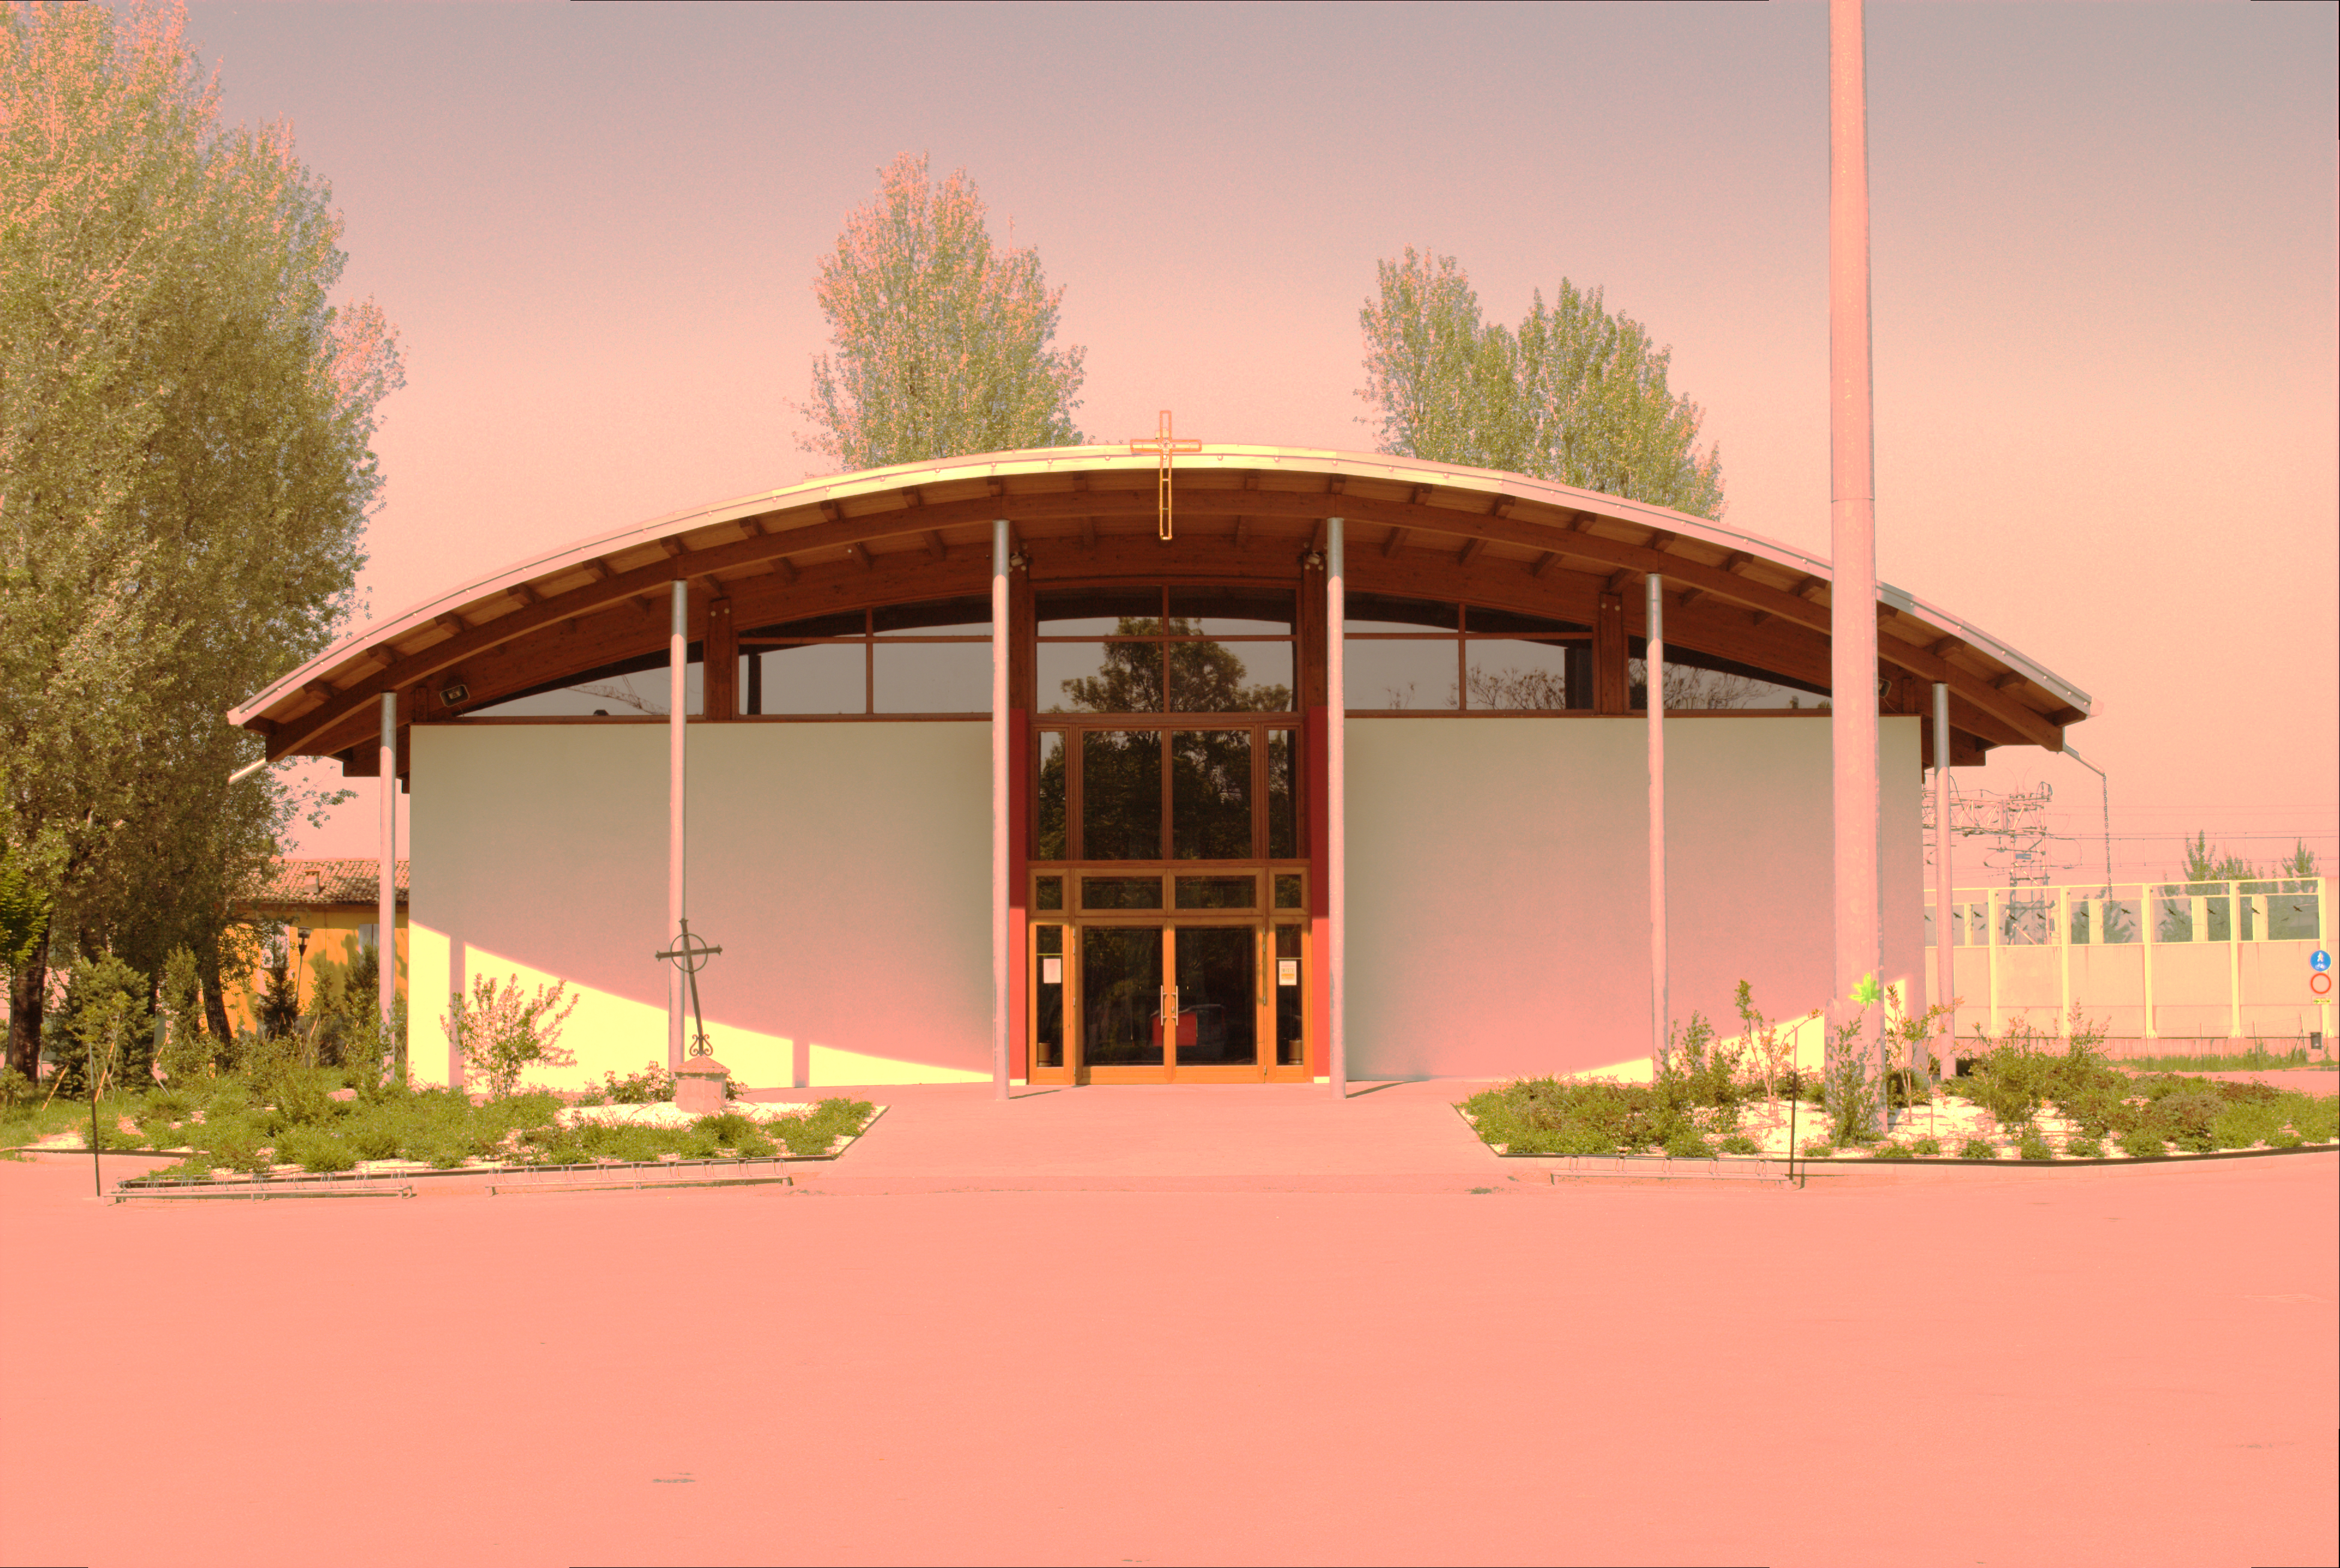
\includegraphics[width=2cm, cfbox=red!50 0.5pt 0pt, trim={35cm 7cm 35.5cm 0cm}, clip, width=11.8cm]{8-our-church.jpg}
\end{figure}
\end{center}

\vspace{-1cm}

% Il prossimo comando aggiunge i ringraziamenti in italiano o in inglese sul retro di copertina
%%%
% The next command adds some acknowledgements in Italian or in English on the back cover
\iftoggle{italianlanguage}{\vspace{3mm}Grazie alle nostre famiglie, agli amici, a don Adriano, a tutti i ministri,\\
 ai ministranti e al Coro San Silvestro della parrocchia di Crevalcore.}{}
\iftoggle{englishlanguage}{Special thanks to our families, to our friends, to don Adriano, to all\\
 the churchmen, to the ministers and to the Choir ``Saint Sylvester''\\
 of the parish of Crevalcore.}{}

% At last, we're done! Enjoy your wedding!
 \end{document}
} % Questo chiude la seconda espressione condizionale % This closes the second conditional form above
} % Questo chiude la prima espressione condizionale % This closes the first conditional form above